\documentclass[a4paper,12pt, notitlepage]{article}

\usepackage[top=25mm,bottom=25mm,left=25mm,right=25mm]{geometry}
%\usepackage{cite}
\usepackage{amsmath} 
\usepackage{graphicx}
\usepackage{epstopdf}
\usepackage{mathtools}
\usepackage{subcaption}
\usepackage{url}
\usepackage{setspace} 
\setstretch{1.44}
\setlength{\columnsep}{6mm}
\usepackage{titlesec}
\usepackage[version=3]{mhchem}
\usepackage{gensymb}
\titleformat{\section}{\bfseries\large\scshape\filcenter}{\thesection}{1em}{}
\titleformat{\subsection}{\bfseries\normalsize\scshape\filcenter}{\thesubsection}{1em}{}

\renewcommand{\abstractname}{}    % clear the title
\newcommand{\captionfonts}{\footnotesize}
\renewcommand\thesection{\Roman{section}.}
\renewcommand\thesubsection{\Alph{subsection}}

\makeatletter
\long\def\@makecaption#1#2{
  \vskip\abovecaptionskip
  \sbox\@tempboxa{{\captionfonts #1: #2}}%
  \ifdim \wd\@tempboxa >\hsize
    {\captionfonts #1: #2\par}
  \else
    \hbox to\hsize{\hfil\box\@tempboxa\hfil}%
  \fi
  \vskip\belowcaptionskip}

\renewcommand\p@subsection{\thesection}
%\additional modules I loaded-------------------------
\makeatother

\usepackage[sorting=none]{biblatex}
\addbibresource{bibliography.bib}

\addbibresource{bibliography.bib}
\usepackage{easyReview}
\usepackage{cleveref}
%\----------------------------------------------------
\begin{document}

\title{\textbf{\large{Final Year Physics Project – Final Report}}}

\author{\normalsize{1803982} \\
        \small\textit{
        Department of Physics, University of Warwick,
        Coventry CV4 7AL, United Kingdom}}
\date{}
\maketitle
\vspace{-10mm}

\begin{abstract} 
\noindent
In this report, an experimental proposition is explored on how the mass of a neutrino may be detected and measured due to the phenomenon of beta decay in Tritium atoms. In particular, simulations are performed in order to ascertain the feasibility of the experiment hypothesised in a practical environment. The results obtained demonstrate that electron trapping in a magnetic bathtub trap with a cloud of Tritium atoms may be an alternative method to its contemporaries such as the KATRIN and Project 8 collaborations.
\end{abstract}
\vspace{6mm}

\section{Project Introduction}
%\textbf{(i) a section stating the overall aims and objectives of your project and setting them in a general context (i.e., giving the “bigger picture”).  In other words, state the problem you are trying to solve in your project and why it is important:} \smallskip \\
In modern particle physics the determination of the neutrino mass from experimental data has been one of the most important challenges of the field. The value of the neutrino mass is of great importance because it plays a decisive role in many assumptions and constructions of modern physical theories. The Standard Model initially assumed the neutrino to be a massless particle, but with the advent of modern experiments a lower limit for the mass of a neutrino has been discovered \cite{Formaggio2021}. As a result, the existence of neutrinos with nonzero mass has encouraged a re-evaluation of the Standard model. Another example of the importance of the nonzero mass of the neutrino relates to the field of cosmology, in which it has been discussed that massive neutrinos may play a significant role in the history of
the Universe \cite{Lesgourgues2006}.
Pauli was the first to estimate the mass of the neutrino. In his letter titled ‘Dear Radioactive Ladies and Gentlemen’ Pauli offered an upper bound for the neutrino mass, stating ‘The mass of the neutron should be of the same order of magnitude as the electron mass and in any case not larger than 0.01 times the proton mass.’ \cite{Pauli1930}.
The prediction, however, was much larger by many orders of magnitude. By the end of 1990, the upper bound for the mass of the neutrino was redefined to several electron-volts (much smaller than Pauli’s 10 MeV bound - 1 percent of the proton mass). Although works to redefine the upper bound had been published throughout the 20th century, it was not until the late 1990s that the existence of a nonzero neutrino mass was reported. 
In 1998, the Super-Kamiokande collaboration gave conclusive evidence for the existence of nonzero neutrino mass. This was aided by the discovery of atmospheric neutrino oscillations \cite{SuperKamiokande1998}, which resulted in accurate measurements of neutrino mass-squared differences ($\Delta m_{21}^{2} \equiv m_{2}^{2} - m_{1}^{2}$, for two different neutrinos of mass $m_{1}$ and $ m_{2}$). Unfortunately, oscillation experiments are unable to measure the mass of individual neutrinos, so new experiments based on alternative observables dependent on non-zero neutrino masses had to be devised. As the relationship between the observables and the neutrino mass has not always been explicit, theoretical foundations had to be employed in order to determine the neutrino mass from the observables measured. One particular observable of interest is the energy spectrum produced by beta decay or electron capture. By analysing the energy spectrum of these processes (a method dating back to Enrico Fermi's conceptualisation of radioactive decay) \cite{Fermi1938}, the neutrino mass may be accessed directly by performing kinematic measures.
The phenomenon of nuclear beta decay is of paramount importance in the project discussed, specifically tritium beta decay, and will be explained in more detail later. Groups such as KATRIN (Karlsruhe Tritium Neutrino experiment) \cite{Arenz2016}, Project 8 \cite{Project82017} and Quantum Technologies for Neutrino Mass (QTNM) make use of tritium beta decay to accurately measure the neutrino mass. In this report, the experiment that is modelled and discussed is associated with QTNM, but the other aforementioned experiments are of relevance for their similarities and conceptual background, which will be referred to in order to explain the project of the QTNM collaboration. 
\\
\indent The project discussed aims to gain a deeper understanding of magnetostatic trapping of electrons. Computer simulated experiments will be conducted to model magnetostatic traps for electrons and simulate the trajectories and cyclotron radiation of free electrons in these traps. As The QTNM collaboration was very recently established, this report's goals have shifted during the production of this report in order to follow recently established results. The modelling results obtained in the present work might support current plans on building and performing the physical experiment, and will report the practical feasibility of detecting the power of an electron.
%\textbf{(ii) an account of the background theory to the work you have been doing.  If you are doing an experimental project, this could be the theory underlying the experimental technique or data analysis methods you are using.  If a theoretical project, this might be a description of the theoretical approach you are using and developing.  If computational, it will ideally be the underlying theory relating to the Physics problem for which your program is being written.} 
%------------------------------------------------------------------------
%------------------------------------------------------------------------
%------------------------------------------------------------------------
%------------------------------------------------------------------------
%------------------------------------------------------------------------
\section{Background Theory}
%------------------------------------------------------------------------
\subsection{Beta Decay}
In beta decay, a `parent' nucleus disintegrates into a `daughter' nucleus via emission of a beta particle and an antineutrino. (see \cref{fig:fig01}).
Beta decay releases energy from the process, which is carried away by the daughter nucleus, the electron (beta particle) and neutrino. The mass of the daughter nucleus is larger than the mass of the electron and neutrino by many orders of magnitude. Therefore, the kinetic energy of the daughter nucleus is considered to be negligible. Consequently, the electron and the neutrino share the decay energy released in variable proportions, which depend on statistics developed from quantum mechanics. The overall energy released is called the Q-value, which can be calculated from the nuclear mass difference of the reactants and the products at rest (see \cref{eq:1} ). The Q-value is usually expressed in MeV. 
For example, in a decay reaction involving a parent particle $A$ which produces particles $b$ and $B$, the Q-value is calculated as \cite{zuber2011neutrino}:
\begin{equation}\label{eq:1}
    Q = \left[\left(m_A\right) – \left(m_b + m_B\right)\right]\,c^{2}
\end{equation}
where $m_a$ is the mass of projectile $a$, $m_A$ the mass of particle $A$, $m_b$ the mass of particle $b$, $m_B$ the mass of particle $B$, and $c$ is the speed of light in a vacuum. The equation is based on Einstein's mass-energy equivalence $E = m c^{2}$, where the mass $m$ here is the difference in mass of reactants and products. When considering beta decay, the reaction does not include a projectile particle $a$. Moreover, in beta decay the disintegrating nucleus is referred to as the parent nucleus and the product nucleus is called the daughter nucleus. 

\begin{figure}[hbt!]
\centering
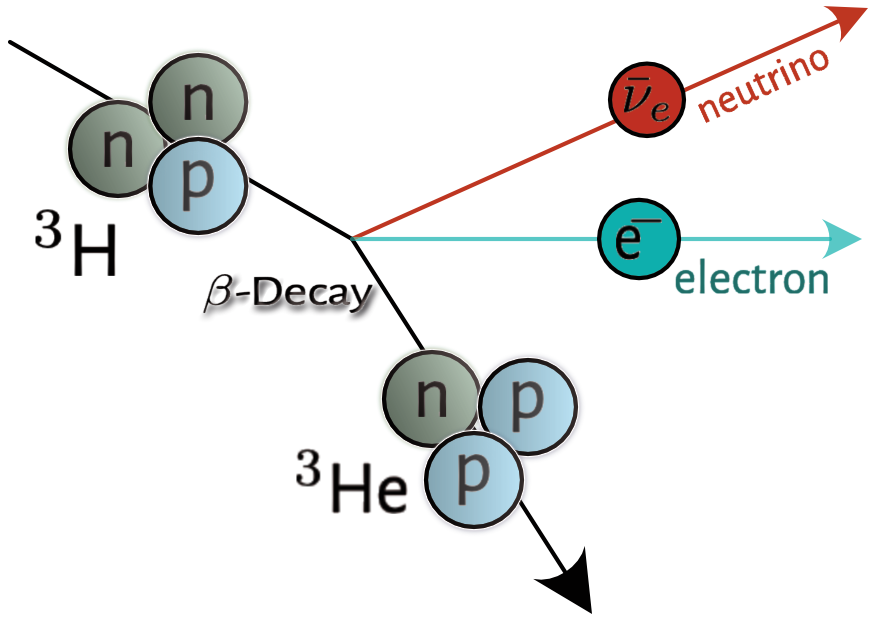
\includegraphics[width=77mm]{pictures/betaDecay.png}
\vspace{-2mm}
\caption{Beta decay of a tritium atom into Helium. Figure based on the KATRIN experiment \cite{steidl} and produced in image processing software.}
\label{fig:fig01}
\end{figure}

Beta emission has a characteristic distribution of energy, called the beta spectrum \cite{Knoll2010}, which can be used to calculate the energy carried by the neutrino. Considering both the law of conservation of energy, and the equivalence between energy and mass ($E = m c^{2}$), the electron cannot possess all of the released energy if the neutrino has nonzero rest mass. The energy that the neutrino takes alters the beta energy spectrum near the endpoint. As it is shown in \cref{fig:fig02}, the energy value at the endpoint is lower if the neutrino has nonzero mass (shown as the red curve in \cref{fig:fig02}). The difference in the energy between the two endpoints discussed above has been experimentally calculated to an upper bound of 1 eV. The upper bound value has been re-evaluated since the first experiments to calculate it in the 1950s \cite{Reines1953}.

\begin{figure}[hbt!]
\centering
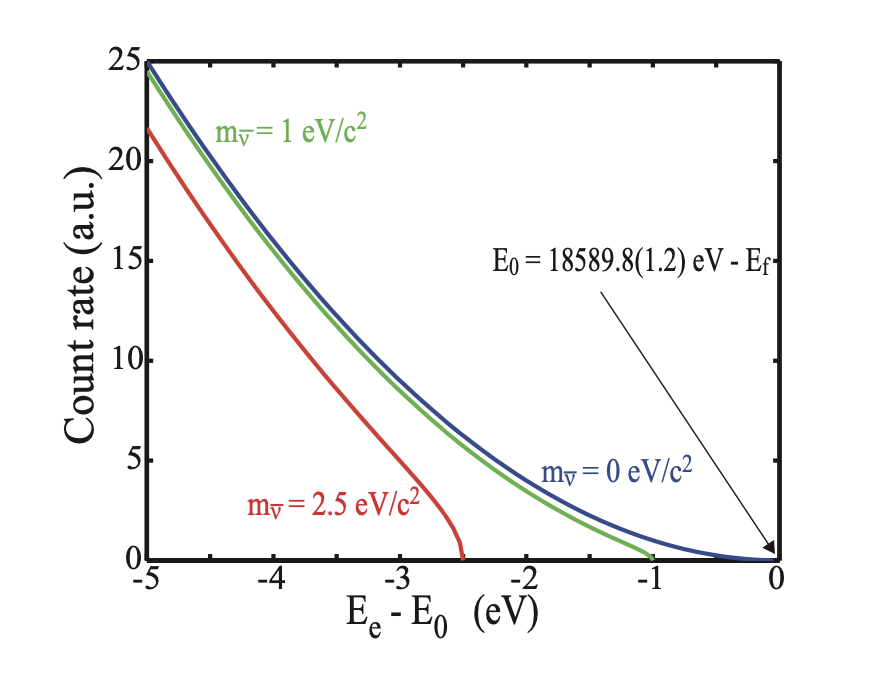
\includegraphics[width=77mm]{pictures/betaDecaySpectrum.png}
\vspace{-2mm}
\caption{Energy spectrum of an electron from tritium beta decay. The endpoint energy is shown to shift down when a non-zero mass $m_{\nu}$ neutrino is emitted. Figure obtained from \cite{Diehl2011}}
\label{fig:fig02}
\end{figure}

As stated previously, the neutrino mass affects the shape of the beta spectrum only near the endpoint. Therefore, in this project the focus is on analysing the spectrum only at the endpoint. Considering the enhanced region of the spectrum near endpoint, it can be seen from \cref{fig:fig02} that the energy spectrum rises quadratically from the endpoint. In a region of energy width $m_{\beta}$, the proportion of decays that produce observable events scales as $(m_{\beta}/Q)^{3}$ \cite{Formaggio2021}. Hence, a low Q-value is desirable in order to maximise the fraction of decays that falls into the endpoint region. Maximising the fraction of decays is beneficial for experiments because they can be less stringent on statistics, suppression, and energy resolution \cite{Kopp2010}. However, the use of an isotope (from any element with isotopes) that has a low Q-value does not guarantee a good basis for an experiment.
In particular, Tritium has a Q-value of 18591 eV and has been the isotope of choice to search for the mass of the neutrino for the last 70 years. Although Tritium's Q-value is large when compared to other beta decay isotope candidates (see \cref{tab:tab1}), its simple nuclear structure requires no nuclear energy dependent corrections applied to the beta emission spectrum, which simplifies the calculation of the spectrum endpoint. Consequently, an important factor in choosing an element isotope is the simplicity in their nuclear structure. A simpler isotope, such as tritium, will produce less background noise due to atomic and molecular effects on the endpoint of the beta decay spectrum.
%Nonetheless, the low endpoint energy in Tritium's beta energy spectrum implies that the total effect of neutrinos on the energy spectrum is more significant than on other energy spectra of different element isotopes.
Another important factor is the specific activity of the source. Specifically, tritium's half life of 12.3 years means that a relatively smaller source mass is required for beta decay experiments when compared to other element isotope candidates (see \cref{tab:tab1}). Moreover, tritium undergoes superallowed beta decay, in which the quantum-mechanical wavefunction of the entire nucleus is left unchanged by the beta decay process (with the exception of one neutron being converted into a proton, as shown in \cref{fig:fig01}). Hence, superallowed beta decay makes tritium an ideal isotope for theoretical analyses \cite{Hardy2012}.
In order to measure the energy of the electrons emitted from a tritium atom, the electrons must be contained in a controlled environment where we can predict the electron's motion. The phenomenon of electron cyclotron resonance (ECR) is employed to determine an electron's trajectory in a magnetic field. The electron's motion can be influenced by the use of magnetic traps, so that an electron under cyclotron resonance can be restrained inside of a desired volume.

\begin{table}
    \centering
    \begin{tabular}{|c|c|c|c|c|c|}
    \hline
    Isotope & Half-life & Specific Activity & Q-value & Source Mass \\
      & (years) & (Bq/g) &  & (g)  \\
    \hline\hline
    \ce{H2^{3}} & 12.3 & $3.6 \times 10^{14}$ & 18591 & $2.0 \times 10^{-7}$\\
    \hline
    \ce{In^{115}} & $4.4 \times 10^{14}$ & 0.26 & 155 & $7.5 \times 10^{7}$\\
    \hline
    \ce{Cs^{135}} & $1.5 \times 10^{6}$ & $6.8 \times 10^{7}$ & 440 & 0.4 - 217\\
    \hline
    \ce{Re^{187}} & $4.3 \times 10^{10}$ & $1.6 \times 10^{3}$ & 2470 & 57 \\ 
    \hline
    \end{tabular}
    \caption{Table of element isotopes comparing their half-lives, specific activity, Q-value and required source mass. Table obtained from \cite{Formaggio2021}}
    \label{tab:tab1}
\end{table}
%------------------------------------------------------------------------
%------------------------------------------------------------------------
%------------------------------------------------------------------------
%------------------------------------------------------------------------
%------------------------------------------------------------------------
\subsection{Magnetostatic Traps}
Electron cyclotron resonance states that a free electron will move in ideal circular motion under the influence of a uniform magnetic field, where the motion of the electron can be described by the Lorentz Force:
\begin{equation}
    \vec{F} = q(\vec{E} + \vec{v} \times \vec{B})
\end{equation}
for a charge of the particle $q$ and $\vec{E}$ the electric field, $\vec{v}$ the charge's velocity, and $\vec{B}$ the magnetic field all calculated at the particle's position at some time.
If the electron's velocity has a non-zero component in the $z$ (or axial) direction, then superposition of this component with the circular motion results in a helical trajectory, see \cref{fig:fig03}.

\begin{figure}[hbt!]
\centering
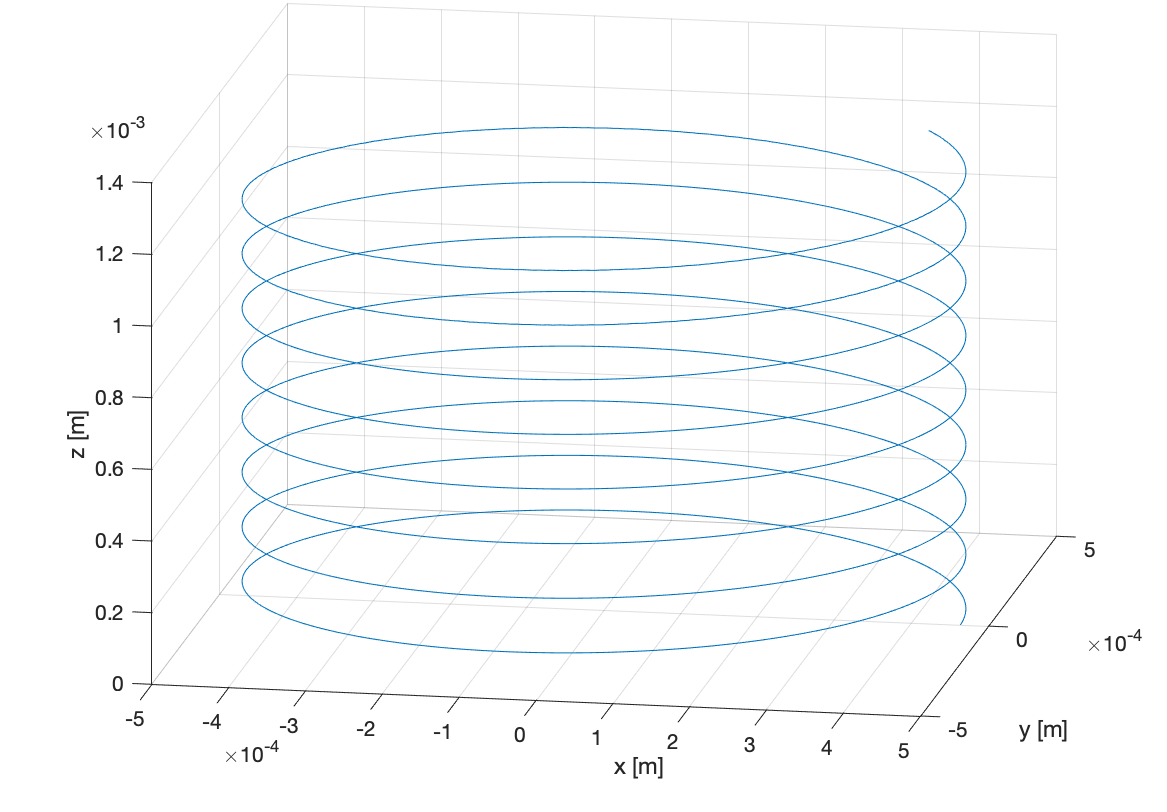
\includegraphics[width=0.6\textwidth]{pictures/idealCyclotronMotion.png}
\vspace{-2mm}
\caption{Ideal helical trajectory of an electron under the Lorentz Force. The pitch angle here refers to the angle of the velocity with respect to the local magnetic field. A uniform 1 T magnetic field pointing in the $z$-axis is considered in this figure. Figure obtained through personal code.}
\label{fig:fig03}
\end{figure}

The magnetic traps applied by the QTNM project are composed of a homogeneous 1 T field superimposed with two solenoid coil fields at each end of a cylindrical volume, called a bathtub or bottle trap. The solenoid coils included deliberately distort the uniform magnetic field \cite{Brown1986}, in order to invert an electron's motion in the $z$-direction. Defining the pitch angle of an electron as the angle between its momentum and the local magnetic field, the equation for an electron's magnetic moment is given by \cite{Ashtari2019}:
\begin{equation}
    \mu(t) = \frac{1}{2}\frac{p_{0}^{2}}{m_{e}}\frac{\sin^{2}(\theta(t))}{B(t)}
\end{equation}
for $p_{0}$ the magnitude of the electron's momentum, $m_{e}$ the electron's mass, $B(t)$ the magnetic field, and $\theta(t)$ the pitch angle. This magnetic moment is constant when the magnetic field direction changes slowly compared to the cyclotron (angular) frequency.

As electrons approach the distortions applied on the magnetic field, this pitch angle approaches $90 \degree$ because the magnetic moment associated with the electron couples to the bottle field \cite{Brown1986}. The electron's axial motion is inverted when the pitch angle reaches $90 \degree$, and the electron then undergoes cyclotron motion in the opposite axial direction, overall trapping the electron in a region of uniform magnetic field.
By defining a new pitch angle $\theta_{bot}$ as the pitch angle in the homogeneous region of the magnetic trap, a restraint can be imposed on the new angle by conservation of energy \cite{Ashtari2019}:
\begin{equation} \label{eq:pitchAngleCondition}
    \theta_{bot} \geq \sin^{-1}\left(\sqrt{1 - \frac{\Delta B}{B_{max}}}\right)
\end{equation}
where $\Delta B$ is the depth of the magnetic trap, and $B_{max}$ is the maximum magnitude of the magnetic field, in Tesla.
If an electron has a pitch angle smaller than this limit, it cannot be restrained in the bathtub trap because it's kinetic energy in the axial direction is large enough to overcome the potential well imposed by the trap.
As the electron undergoes cyclotron motion inside the magnetic trap, it will radiate power through electromagnetic radiation, determined by the Lienard-Wiechert equations for a relativistic-ally moving point charge \cite{Jackson1999}. In order to measure the electron's energy from its power radiated, the method of cyclotron radiation emission spectroscopy (CRES) is employed.
%------------------------------------------------------------------------
%------------------------------------------------------------------------
%------------------------------------------------------------------------
%------------------------------------------------------------------------
%------------------------------------------------------------------------
\subsection{Cyclotron Radiation Emission Spectroscopy}
Electrons trapped in the magnetic trap undergo cyclotron motion with a cyclotron frequency $\Omega_{c}$ that depends on the kinetic energy $K_{e}$ of the electron, given by \cref{cyclotronFrequency} \cite{Monreal2009,Ashtari2019,Asner2015}:
\begin{equation} \label{cyclotronFrequency}
    \Omega_{c} = \dfrac{\Omega_{0}}{\gamma} = \dfrac{qB}{m_{e} + K_{e} / c^{2}} 
\end{equation}
Here, $\Omega_{0}$ is a non-relativistic frequency, $\gamma$ is the electron's Lorenz factor, $q$ the elementary charge of an electron, $m_{e}$ the mass of the electron and $B$ the applied magnetic field.
At a known value of $B$, the kinetic energy of electrons emitted in beta decay can be determined by measuring the cyclotron frequency \cite{Asner2015}.  

In order to understand how the cyclotron frequency can be determined, an additional concept must first be established. Specifically, emission of electromagnetic radiation by the electron. It has been established since 1897 that accelerating charges emit electromagnetic radiation \cite{Larmor1897}. An electron moving in cyclotron motion emits a particular form of radiation aptly named cyclotron radiation. Cyclotron radiation, which was first derived in 1904 \cite{Heaviside1904}, has been used to indirectly detect single electrons with cyclotron motion in magnetic traps \cite{VanDyck1977}. The cyclotron radiation emitted by an electron produces a power spectrum that has a central peak at exactly the average cyclotron frequency $\Omega_{c}$ of the electron \cite{Asner2015, Monreal2009} (see \cref{fig:fig04}). In other words, the cyclotron frequency could be obtained from the central peak in the power spectrum of the radiation. The central peak is deduced to be the average cyclotron frequency because most of the power emitted occurs at the average frequency. \\
Since the cyclotron frequency and the energy of an electron are related to one another, the power emitted by the electron will cause a slight shift in the electron's frequency over time. However, the power emitted by the electron is not too large such that the electron's energy is quickly changed \cite{Monreal2009}, and as such the power emitted can be approximated as a constant for small periods of times \cite{Ashtari2019}. With this approximation, an equation for the frequency at a given time can be extracted from \cref{cyclotronFrequency}, \cite{Ashtari2019}: 
\begin{equation}
    \Omega_{c}(t) \approx \dfrac{qB(t)}{m_{e} + K_{0} / c^{2}} \left( 1
    + \dfrac{Pt}{m_{e}c^{2} + K_{0}}\right)
\end{equation}
This approximation allows the energy of the electron to be indirectly measured without any detriment to the accuracy of the calculations. Hence, the cyclotron radiation emission spectroscopy is referred as nondestructive spectroscopy. 
Frequency-based spectroscopy (such as CRES) overcomes many of the pitfalls of traditional spectroscopic methods (for example, in direct neutrino mass experiments involving tritium). Traditional spectroscopic techniques are limited by the need to extract the beta decay electron for measurement. Such a requirement imposes a practical limitation on the size and density of the tritium source used, because electrons would be harder to extract from tritium gas. However, tritium gas is transparent to cyclotron radiation, so the size and density of the tritium source is irrelevant to cyclotron radiation emission spectroscopy \cite{Asner2015}. \\

\begin{figure}[b!]
\centering
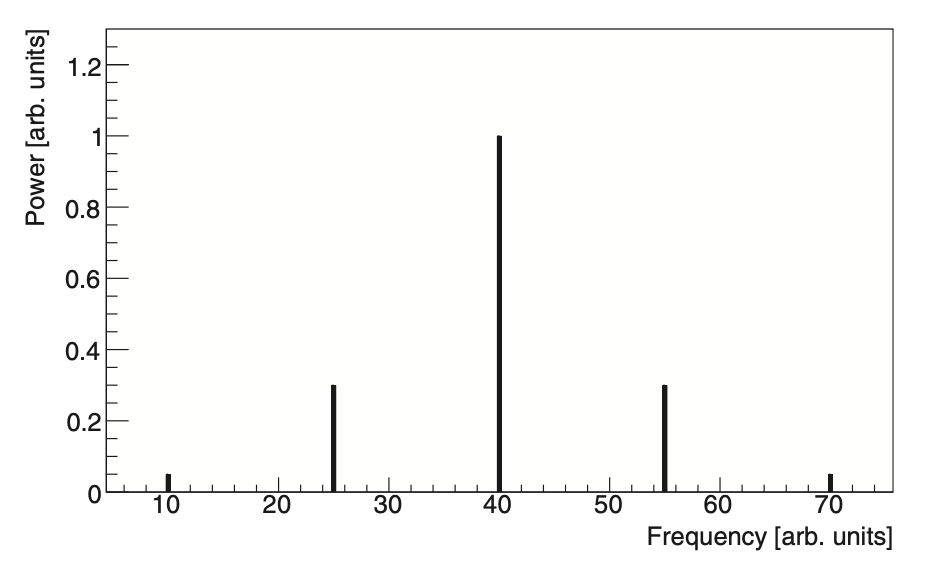
\includegraphics[width=0.6\textwidth]{pictures/powerSpectrum.png}
\vspace{-2mm}
\caption{Frequency spectrum of the cyclotron power from an electron in a 1-T magnetic field with an energy of 30keV. The peak frequency at 40MHz (the central peak) is the average cyclotron frequency after down-mixing.  Down-mixing the signal must be performed so that the signal can be digitised, as there are no digitisers for signals with magnitudes of 10 GHz. The separation between the peaks after down-mixing (called the axial frequency), is 15 MHz . Figure obtained from \cite{Ashtari2019}}.
\label{fig:fig04}
\end{figure}
For an electron in mildly relativistic motion around a 1 T background field, the power radiated is of the magnitude of femtowatts ($10^{-15}$ W) \cite{Ashtari2019}. This poses a particular obstacle in detecting the radiation of the electron over the background white noise due to the thermal phenomena of electrical equipment, called the Johnson-Nyquist noise. 
The noise is described by a Gaussian normal distribution and the noise power is given from the equipartition theorem \cite{Nyquist1928} by \cite{Kittel1980, reif1965}:
\begin{equation}
    N = k_{B}T\Delta f
\end{equation}
for $k_{B}$ the Boltzmann constant, $T$ the circuitry in Kelvin, and $\Delta f$ the bandwidth of the noise in Hertz. The Johnson-Nyquist noise is many orders of magnitude larger than the power radiated from the electron, even at a temperature of 4K, so to be able to detect the electron's power radiation an instrument called a lock-in amplifier must be utilized. Lock-in amplifiers are discussed in \cref{amplifier}.
A final consideration in measuring cyclotron radiation includes the application of antennas. Antennas are the main equipment in receiving the power of the radiation, and as such must be included in our experiment for the measurement of power radiated.
%------------------------------------------------------------------------
%------------------------------------------------------------------------
%------------------------------------------------------------------------
%------------------------------------------------------------------------
%------------------------------------------------------------------------
\subsection{Antenna Theory} \label{antenna}
As mentioned above, antennas are used to receive the power emitted by beta decay electrons. In modelled experiments the beta decay electron must be assumed to act as a transmitting antenna (with power transmitted $P_{T}$). The power transmitted by a non-relativistic moving charge was derived from the Lienard-Wiechert radiated fields \cite{Jackson1999}, producing the Larmor formula \cite{Larmor1897-2}. A generalisation of the Larmor equation, to consider the total radiated power of a relativistic charge, was derived by Lienard in 1898. Thus, for a relativistic point charge the total power radiated is given by \cref{eq:3} \cite{Griffiths.2009}.
\begin{equation} \label{eq:3}
    P_{T} = \dfrac{\mu_{0} e^{2}}{6 \pi c} \left(a^{2} - \left(\dfrac{\boldsymbol{v} \times \boldsymbol{a}}{c}\right)^{2}\right)
\end{equation}
Here, $\mu_{0}$ is the permeability of free space, $e$ is the elementary charge of an electron, $c$ is the speed of light, $\boldsymbol{v}$ is the velocity of the charge and $\boldsymbol{a}$ is its acceleration.
In the case of cyclotron motion, the velocity is orthogonal to the acceleration (with $a = \dfrac{e v B}{\gamma m_{e}}$), thus \cref{eq:3} simplifies to: 
\begin{equation} \label{eq:4}
    P_{T} = \dfrac{\mu_{0} e^{2} \Omega_{c}^{2} v^{2}}{6 \pi c}\gamma^{4}
\end{equation}
for a cyclotron frequency $\Omega_{c} = (e\,B)/(\gamma m_{e})$. \\
Once the power transmitted has been determined, the power received $P_{R}$ at an antenna of distance $R$ may be obtained using the radio equation \cite{Visser2012}.
\begin{equation}
    \dfrac{P_{R}}{P_{T}} = \left(\dfrac{\lambda}{4 \pi R} \right)^{2} G_{R} G_{T}
\end{equation}
Here, $\lambda$ is the wavelength of the radiation emitted, and $G_{R}$, $G_{T}$ are the gains of the receiving and transmitting antenna respectively.
The gain of an antenna gauges how much power the antenna can transmit/receive in any direction. The gain $G(\theta,\phi)$ is dependent on the polar $\theta$ and azimuthal $\phi$ angles around the antenna (see \cref{fig:fig05}). Different antenna configurations have different gain geometries which make the structure of the antenna an important factor when considering their applications. In consequence, the antennas employed in the modelling experiment must be carefully considered. The antennas should receive enough power from the electrons in the magnetostatic trap because the power received must be large enough to be differentiated from the background noise. \\

\begin{figure}[t!]
\centering
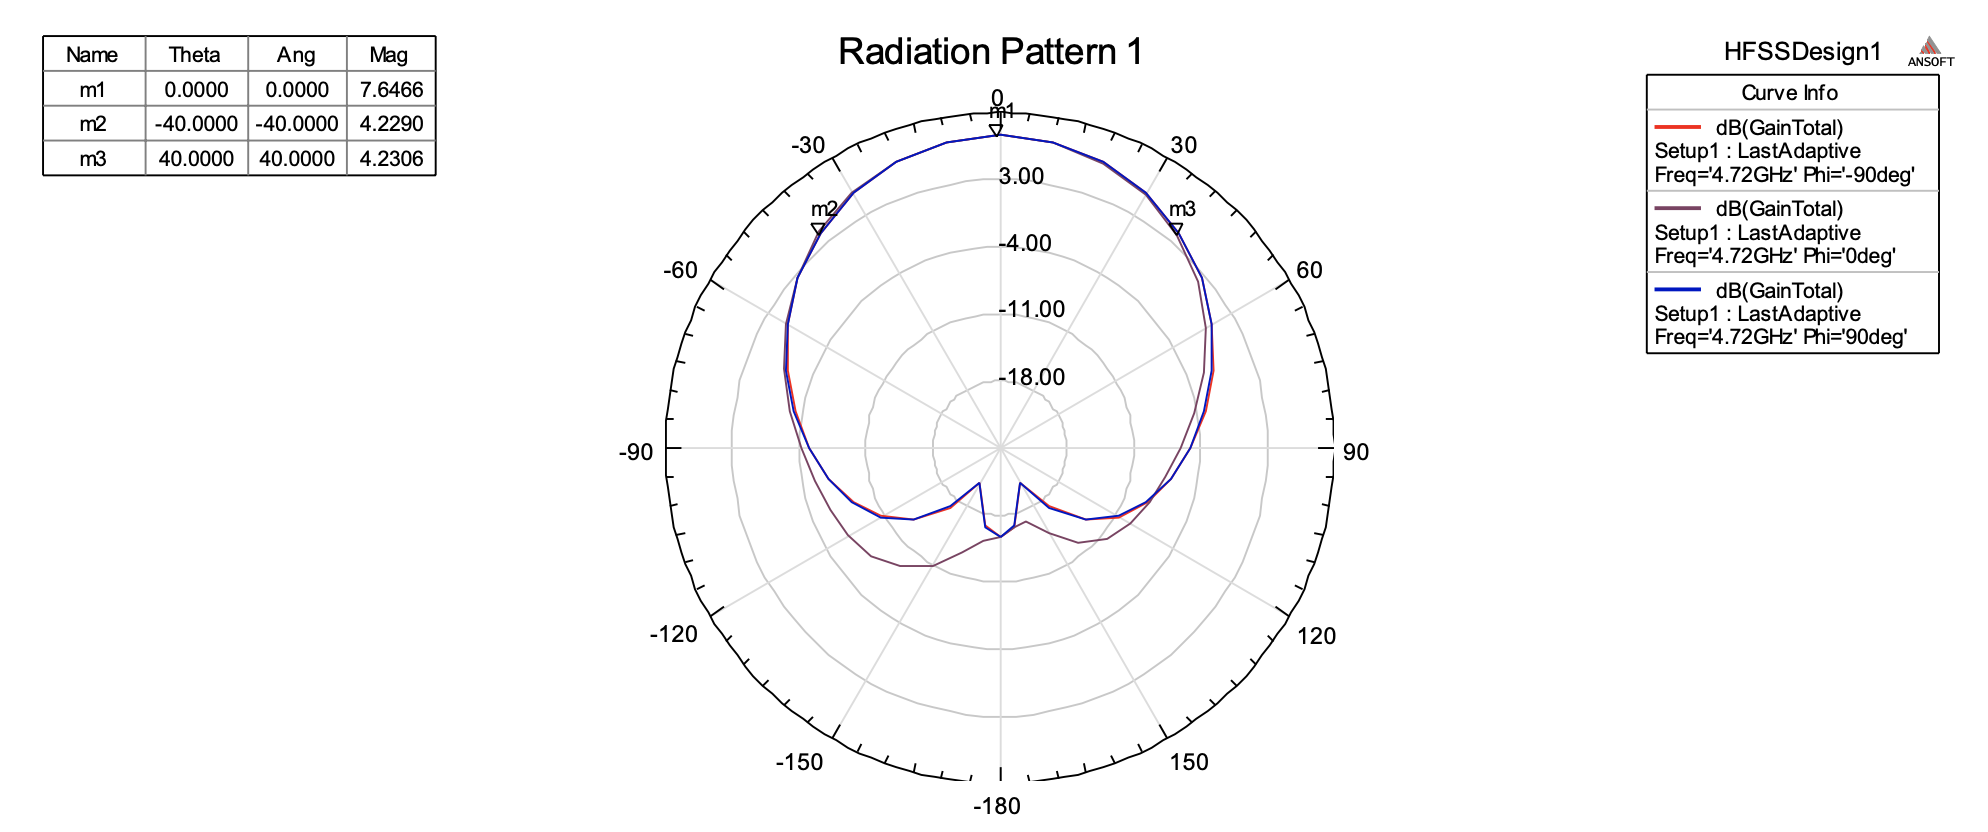
\includegraphics[width=0.7\textwidth]{pictures/gainExample.png}
\vspace{-2mm}
\caption{Example of the gain geometry of an antenna. Figure obtained from \cite{Farahani2008}}
\label{fig:fig05}
\end{figure}
Once an antenna has been modelled to receive the power from an accelerating relativistic electron, we can consider the noise detected from the signal due to the resistance in the electrical circuitry. For simplicity, we can consider the antenna as an equivalent resistor with the same temperature that the antenna will operate at, a temperature of 4 Kelvin.
%------------------------------------------------------------------------
%------------------------------------------------------------------------
%------------------------------------------------------------------------
%------------------------------------------------------------------------
%------------------------------------------------------------------------
\subsection{Lock-in Amplifiers} \label{amplifier}
Lock-in amplifiers can detect signals where the signal-to-noise ratio (SNR) is small, $SNR << 1$. The signal-to-noise ratio is defined as the ratio between the average power of a signal and the average power of the background noise:
\begin{equation}
    SNR = \dfrac{P_{signal}}{P_{noise}}
\end{equation}

The fundamental mathematics of a lock-in amplifier is based on Fourier series. Any signal can be expressed as an infinite sum of sine waves with different frequencies, phases and amplitudes. These sine waves are all orthogonal, meaning that when two sine waves are multiplied, their average product over a time period will be 0 unless their frequencies are exactly the same. This process is called down-mixing, as it will reduce the average product of noise over time, whilst conserving the desired signal intact after the operation. Lock-in amplifiers perform this process using a phase sensitive detector (PSD), which down-mixes an inputted signal $V_{sig}$ with a sine wave at the reference frequency, called a reference signal $V_{ref}$, by multiplying the two signals:
\begin{align*}
    V_{psd} & = V_{sig}\sin(\omega_{sig}t + \theta_{sig})V_{ref}\sin(\omega_{ref}t + \theta_{ref}) \\
    & = \frac{1}{2}V_{sig}V_{ref}\left[\cos((\omega_{sig}+\omega_{ref})t + \theta_{sig}+\theta_{ref}) + \cos((\omega_{sig}-\omega_{ref})t + \theta_{sig}-\theta_{ref}) \right]
\end{align*}
The down-mixing process produces two signals, one for the difference in frequencies $\omega_{sig}-\omega_{ref}=0$, and the other for the sum in frequencies $\omega_{sig}+\omega_{ref}=2\omega_{sig}$. A low-pass filter is then applied in order to separate the DC signal from the AC signal at twice the signal frequency.

Low-pass filters can be described generally by an equation called the transfer function, $H(\omega)$. This function determines the amplitude response of the filter with respect to given frequencies $\omega$, suppressing signals with any frequencies outside the desired bandwidth. 
A Butterworth low-pass filter is employed in this report, with a transfer function described by:
\begin{equation}
    H(\omega) = \dfrac{1}{\sqrt{1 + \left(\dfrac{\omega}{\omega_{c}}\right)^{2n}}}
\end{equation}
here $\omega_{c}$ is the cutoff frequency and $n$ is the order of the low-pass filter. Both the cutoff frequency and the order affects the steepness of the amplitude response at the cutoff frequency. The higher the order of the filter, the steeper the frequency response and the more effective that frequencies outside the bandwidth are blocked. A higher order filter has the downside that it takes longer for the step response function to settle, which causes a phase delay \cite{LockinAmpRef01}. When a step response settles, this indicates that the signal has been completely filtered and only the signal in the desired bandwidth remains. Step responses are useful in discovering the envelope distortion of a filtered signal \cite{StepResponseRef}.
Since the Johnson-Nyquist noise power depends on the bandwidth of frequencies measured, a decrease in the bandwidth will increase the signal-to-noise ratio at the cost of a longer measurement time. In the case of a low-pass filter, the bandwidth is determined by the cutoff frequency used $\omega_{c}$. Hence, decreasing the cutoff frequency will lead to a higher signal-to-noise ratio, giving an overall clearer signal at the cost of a longer measurement time, see \cref{fig:fig06}.

\begin{figure}[t!]
\centering
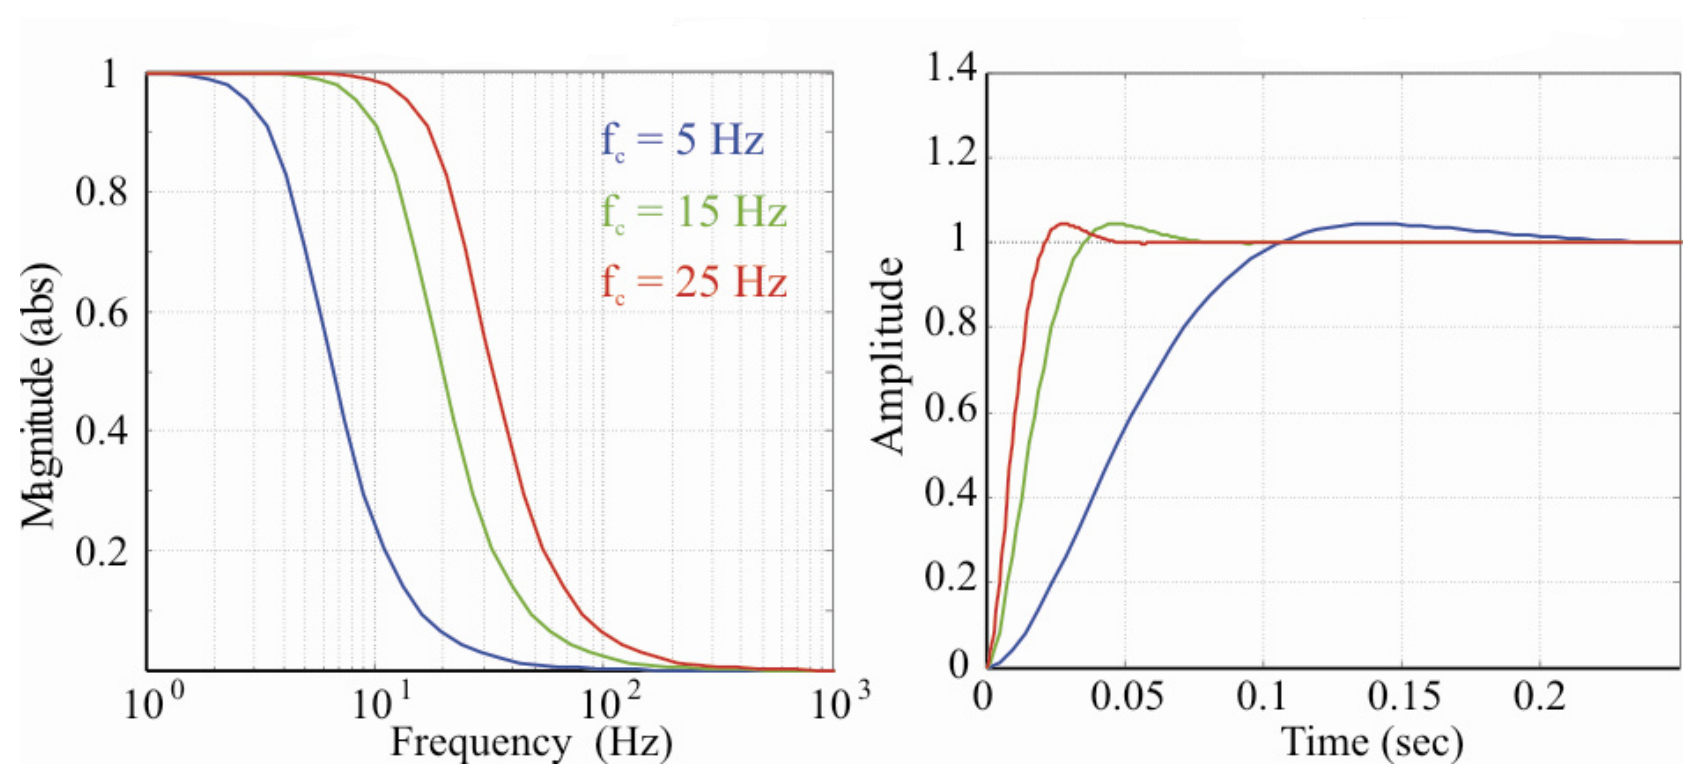
\includegraphics[width=0.8\textwidth]{pictures/butterworthFilter.png}
\vspace{-2mm}
\caption{Plot of the frequency response and the step response of a Butterworth filter for different cutoff frequencies. Figure adapted from \cite{Bula2010}.}
\label{fig:fig06}
\end{figure}
The final step in a lock-in amplifier takes into account the phase dependence on the resulting DC signal, since the resulting output is proportional to the phase difference $\theta=\theta_{sig}-\theta_{ref}$ as $V_{psd} \propto V_{sig}V_{ref}\sin(\theta)$. 
If this phase difference is not exactly 0, then the average product of the desired signal will not be close to 1, which will make the signal harder to detect above the noise. Furthermore, if the phase difference is non-zero our desired signal is no longer DC and may be removed by a low-pass filter with low enough cutoff frequency.
The phase dependency can be removed with the use of a second PSD, which takes advantage of some trigonometric concepts. The second PSD down-mixes the signal frequency with a reference frequency that is phase shifted by $\frac{\pi}{2}$ radians, which is equivalent to multiplying the signal with a cosine reference due to the trigonometric identity, $\sin(\theta+\frac{\pi}{2}) = \cos(\theta)$. 
The two output signals can be defined as $X = V_{psd}\sin(\theta)$, called the in-phase component of the desired signal, and $Y = V_{psd}\cos(\theta)$, called the quadrature component. This terminology is adequate because when $\theta = 0$ $X$ measures the complete signal whilst $Y$ is $0$.
Using Pythagoras' theorem to calculate the magnitude of the signal vector $R$, the signal amplitude can be calculated without any phase dependency between the signal and the reference signals:
\begin{equation}
    R = \sqrt{X^{2}+Y^{2}} = V_{sig}
\end{equation}
Additionally, using the arctangent on the in-phase and quadrature components can provide the phase relationship between the signal and sine reference frequency:
\begin{equation}
    \theta = \arctan\left(\frac{X}{Y}\right)
\end{equation}
As an output, the lock-in amplifier returns both the signal amplitude $R$ and the phase difference $\theta$. A circuit schematic of a lock-in amplifier can be seen in \cref{fig:fig07}

\begin{figure}[t!]
\centering
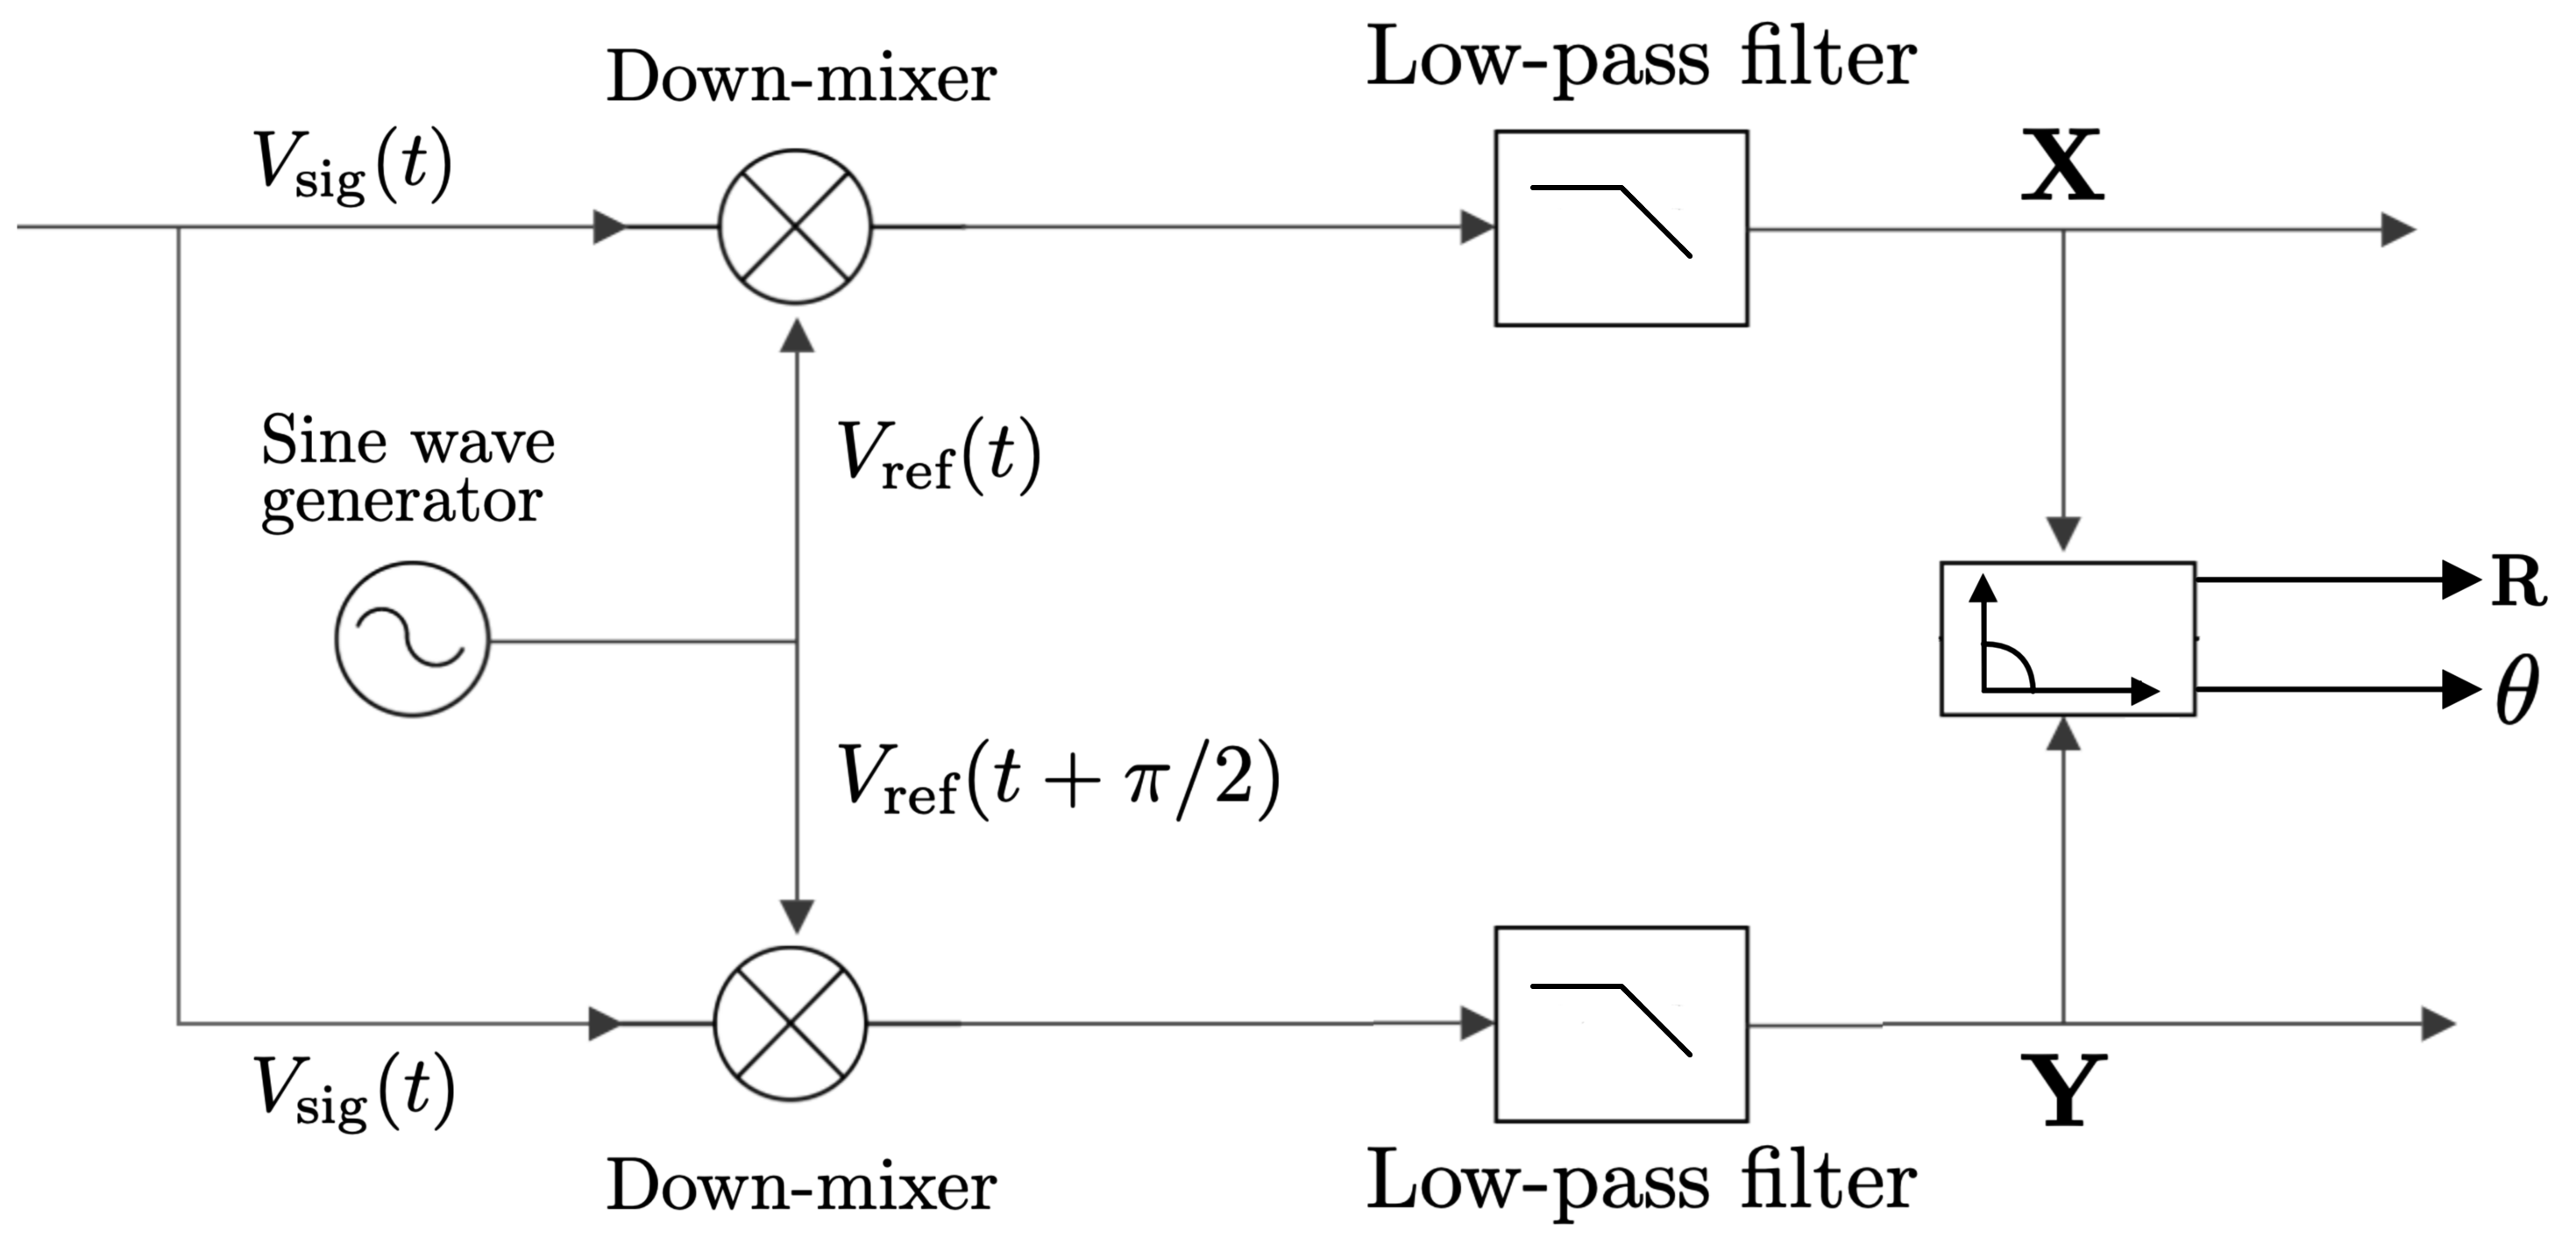
\includegraphics[width=0.8\textwidth]{pictures/diagramCircuit00.png}
\vspace{-2mm}
\caption{Circuit schematic of a lock-in amplifier.}
\label{fig:fig07}
\end{figure}
%------------------------------------------------------------------------
%------------------------------------------------------------------------
%------------------------------------------------------------------------
%------------------------------------------------------------------------
%------------------------------------------------------------------------
\subsection{Summary}
Cyclotron radiation emission spectroscopy can determine the cyclotron frequency of the electron by measuring the frequency of the EM radiation emitted by the electron. The electron's cyclotron frequency may then be related back to the kinetic energy of the electron in order to calculate the endpoint of the beta decay energy spectrum. By computing the difference in the endpoints of the energy spectrum as mentioned previously, accurate results for the mass of the neutrino could be acquired. In order to conduct the experiment and obtain precise results, computer simulations will be performed to understand how a magnetic bathtub trap can be used in conjunction with electron cyclotron resonance to produce electromagnetic radiation that can be measured to determine the electron's kinetic energy. A further consideration will be presented with respect to the noise involved in the experiment, in order to ascertain how lock-in amplifiers may be used to detect a signal within noise that is orders of magnitude larger.
%------------------------------------------------------------------------
%------------------------------------------------------------------------
%------------------------------------------------------------------------
%------------------------------------------------------------------------
%------------------------------------------------------------------------
\section{Computational Tools}
%------------------------------------------------------------------------
%------------------------------------------------------------------------
%------------------------------------------------------------------------
\subsection{Magnetic Bathtub Trap}
The first code that was produced calculated the magnetic field at a position in space and returned the value as a vector $\vec{B} = (B_{x}, B_{y}, B_{z})$. The equations used for this calculation were based on the magnetic field of a circular coil. These values were then superimposed $N$ number of times for $N$ coils around each solenoid, and finally a background field of 1 T was superimposed onto this field to produce the bathtub magnetic trap.

The equation for the magnetic field of a circular coil, at a position $(x,y,z)$ is defined as \cite{Fernow2016}:
\begin{equation}
    B_{r} = \dfrac{I\mu_{0}}{2r}\left[E(\beta)\left(\dfrac{1+\hat{r}^{2}+\hat{z}^{2}}{\gamma}\right) - K(\beta)  \right] \dfrac{1}{\pi\sqrt{\alpha}} \dfrac{z-z_{c}}{R}
\end{equation}
\begin{equation}
    B_{z} = \dfrac{I\mu_{0}}{2r}\left[E(\beta)\left(\dfrac{1-\hat{r}^{2}-\hat{z}^{2}}{\gamma}\right) + K(\beta) \right] \dfrac{1}{\pi\sqrt{\alpha}} \dfrac{z-z_{c}}{R}
\end{equation}

with some variables defined as:
\begin{gather}
    \alpha = (1+\hat{r})^{2}+\hat{z}^{2} \;;\; \beta = \dfrac{4\hat{r}}{\alpha} \;;\; \gamma = \alpha - 4\hat{r}\\
    K(\beta) = \int_{0}^{\frac{\pi}{2}} (1 - \beta^{2}\sin^{2}(t))^{-\frac{1}{2}}dt \;\;;\;\; \textrm{Elliptic integral of the first kind}\\
    E(\beta) = \int_{0}^{\frac{\pi}{2}} (1 - \beta^{2}\sin^{2}(t))^{\frac{1}{2}}dt \;\;;\;\; \textrm{Elliptic integral of the second kind}
\end{gather}

In the equation, $R=\sqrt{x^{2}+y^{y}}$ is the distance of the current position from centre of the coil, or equivalently the distance from the solenoid coil axis. $r$ is the radius of the coil, and $z_{c}$ is the axial position of the coil. $\hat{r}=\frac{R}{r}$ is the distance of the position and $\hat{z}=\frac{z-z_{c}}{r}$ is the axial distance from the the coil to the probed position, both normalised with respect to the coil radius. 
The elliptic integrals were calculated using a two-point Gaussian quadrature method.
%------------------------------------------------------------------------
%------------------------------------------------------------------------
%------------------------------------------------------------------------
%------------------------------------------------------------------------
%------------------------------------------------------------------------
\subsection{Electron Trajectory}
The equation of motion used to calculate the trajectory is given by a linear superposition of the Lorentz force and the radiation reaction force, given by the Abraham-Lorentz equation \cite{Griffiths.2009}. The radiation reaction force considers the motion of rearward thrust due to the power that an electron radiates, by applying Newton's 3rd law. For the code implemented, a reformulation of the Abraham-Lorentz equation given by Ford and O'Connell is employed \cite{Ford1991}:
\begin{equation}
    m_{e}\dfrac{d\boldsymbol{v}}{dt} = q(\boldsymbol{v}\times\boldsymbol{B}) + \dfrac{q^{2}}{6\pi\epsilon_{0}c^{3}m_{e}}\dfrac{d}{dt}\left(q(\boldsymbol{v}\times\boldsymbol{B})\right)
\end{equation}
for $m_{e}$, $q$, $\boldsymbol{v}$ the mass, charge and velocity of an electron respectively, $\boldsymbol{B}$ the magnetic field, $\epsilon_{0}$ the permittivity of free space and $c$ the speed of light. The first term on the right hand side is the Lorentz force, and the second term is the Abraham-Lorentz force. No electric field is included because the electron motion simulated is inside only a magnetic field. To solve these differential equations numerically, the Boris algorithm \cite{Boris1970} is employed to advance an electron in time.
The Boris method is the standard algorithm used in plasma physics simulations due to its outstanding long term accuracy \cite{Hong2013}. This algorithm was used over its contemporaries such as the Runge-Kutta method, because it conserves energy in the system, which is necessary to consider so that the power calculated has no discrepancies due to energy shifts. Additionally, high accuracy in the trajectories is necessary because the power radiated depends on the electron's position, which will alter the measured power significantly since the magnitudes associated are of the order of fW. The Boris method is particularly useful for the computation of the electron trajectories in the project because it only considers the motion due to a magnetic field.
%------------------------------------------------------------------------
%------------------------------------------------------------------------
%------------------------------------------------------------------------
%------------------------------------------------------------------------
%------------------------------------------------------------------------
\subsection{Modelling of Power Radiated}
The power radiated was modelled with two separate codes. The first code employed the Faraday tensor for a moving charge \cite{Jackson1999}:
\begin{equation}
    F^{\mu\nu} = \dfrac{\mu_{0}qc}{4\pi}\left[\dfrac{X^{\mu}\tilde{U}^{\nu}-X^{\nu}\tilde{U}^{\mu}}{cR_{s}^{3}}\left(1 - \dfrac{\vec{X}\cdot\vec{\tilde{A}}}{c^{2}}\right) - \dfrac{X^{\mu}\tilde{A}^{\nu}-X^{\nu}\tilde{A}^{\mu}}{cR_{s}^{2}} \right]
\end{equation}
where:
\begin{gather}
    X = (R,\, \boldsymbol{x} - \boldsymbol{\tilde{x}}) \;\; ;\;\; \textrm{The 4-separation.} \\
    \tilde{U} = \gamma(c,\, \boldsymbol{u}) \;\;;\;\; \textrm{The source's 4-velocity.} \\
    \tilde{A} = \gamma\dfrac{d\tilde{U}}{dt} \;\;;\;\; \textrm{The source's 4-acceleration.} \\
    R_{s} = \dfrac{1}{c}\vec{X}\cdot\boldsymbol{\tilde{U}} = \dfrac{1}{c}X^{\mu}\tilde{U}_{\mu}
\end{gather}
in which a tilde above the vector signifies the variables of the electromagnetic field source, the electron. $R$ is the distance from the observer to the field source, $x$ is the observer position, $\gamma$ is the Lorentz factor and $c$ is the speed of light. 
Using this tensor notation, it becomes easy to read off the electric field $\boldsymbol{E}$ and magnetic field $\boldsymbol{B}$ components of the radiation emitted by the electron. Once the electric and magnetic fields are computed, the Poynting vector $\boldsymbol{P} = \frac{1}{\mu_{0}}\boldsymbol{E}\times\boldsymbol{B}$ is then outputted to find the power radiated at each electron position. \\
 
The second code implemented an equation for the power received due to the Lienard-Wiechert radiation fields of an accelerating charge \cite{Jackson1999}. The equation implemented was derived by calculating the angular distribution of the power due to the Lienard-Wiechert fields in the relativistic case \cite{private1}:
\begin{equation}
    |\boldsymbol{P}(\boldsymbol{\tilde{x}})| = \dfrac{1}{\mu_{0}c}\left[\dfrac{e}{4\pi\epsilon_{0}c^{2}R}a\right]^{2}\dfrac{1}{(1 - \beta\sin\theta)^{3}}\left[1 - \dfrac{\cos^{2}\theta}{\gamma^{2}(1 - \beta\sin\theta)^{2}}\right]
\end{equation}
where $R$ is the distance between the field point and the position of the charge, $a$ is the magnitude of acceleration of the charge, $\theta$ is the angle between the acceleration vector and the unit vector pointing towards the antenna. $\mu_{0}$ is the vacuum permittivity, $\epsilon_{0}$ is the vacuum permeability, $c$ is the speed of light, $e$ is the charge of an electron, $\beta = \frac{v}{c}$ for a speed $v$, and $\gamma$ is the Lorentz factor. 
With the formulation employed, electron trajectories can be inputted as a text file into the codes, and power received can be calculated for a number of positions over some simulation time.
 
Additionally, an observing position is also inputted into the code to find the power measured at an antenna. For simplicity, the gain of the electron's radiated power $G_{T}$ is assumed to be 1, and the antenna considered is a Hertzian dipole. The power received at the antenna is then  $|\boldsymbol{S}(\boldsymbol{\tilde{x}})| = |\boldsymbol{P}(\boldsymbol{\tilde{x}})|A_{e}$, where the effective area for a Hertzian dipole is \cite{Visser2012}: 
\begin{equation}
    A_{e} = \dfrac{\lambda^{2}}{4\pi}G_{R} = \dfrac{3\lambda^{2}}{8\pi}\sin^{2}(\psi).
\end{equation}
The angle $\psi$ is the angle between the separation vector, and the orientation vector of the Hertzian dipole. The value of $\sin^{2}(\psi)$ can be calculated using trigonometric identities and vector operations on the aforementioned vectors. For the simulation involved, the direction of the dipole orientation will be parallel to the angular velocity of the cyclotron motion, so that the antenna receives the most power available from the electron, see \cref{fig:antenaSetup}.
 
\begin{figure}[t!]
\centering
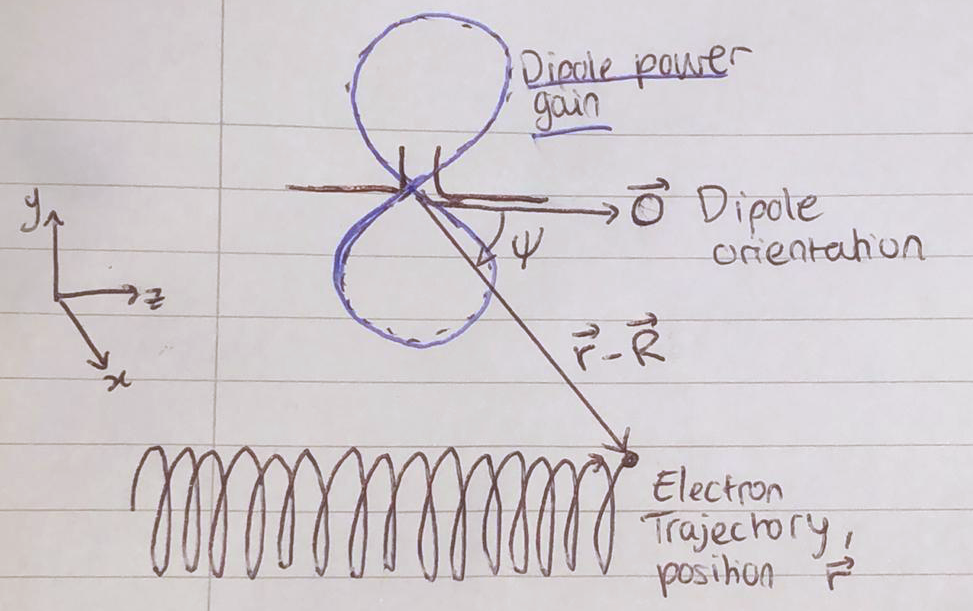
\includegraphics[width=77mm]{pictures/antennaSetup.png}
\vspace{-2mm}
\caption{Vectorial schematic for the position and orientation of the antenna modelled, with respect to the electron trajectory. $\vec{R}$ is the position of the antenna, and $\psi$ is the angle between the separation and the orientation vectors. The orientation $\vec{O}$ is parallel to the z axis.}
\label{fig:antenaSetup}
\end{figure}
%------------------------------------------------------------------------
%------------------------------------------------------------------------
%------------------------------------------------------------------------
%------------------------------------------------------------------------
%------------------------------------------------------------------------
\subsection{Lock-in Amplifier}
In order to simulate the power received at an antenna, a voltage sine wave with the desired frequency was emulated in order to check if the lock-in amplifier was able to detect the signal within some Gaussian noise with variance of $4k_{B}TR$. Python code generated this noise for a temperature $T = 4$ K and a resistance of $R = 0.01\,\Omega$. The signal was emulated as a sine wave because the relationship between power received and the voltage induced is given by the relationship $P = \frac{V^{2}}{R}$. If the signal was simply the square root of the power received, this would result in a voltage with a non-zero time average $\langle V \rangle \neq 0$, which would include a DC component into the voltage inside the antenna. \\
For an electron with energy of 18.575keV, the expected frequency of the signal detected is 27.01GHz, calculated with a reformulation of \cref{cyclotronFrequency}:
\begin{equation}
    f = \dfrac{qBc^{2}}{2\pi(E + mc^{2})}
\end{equation}
where the $2\pi$ factor comes from the relationship between frequency and angular frequency. 
A lock-in amplifier assumes that the frequency of the signal is already known before applying the amplifier in order to detect the signal frequency desired. Since there is only an upper limit on the mass of a neutrino as the closest estimate to the mass, the exact frequency related to the electron emitted is not yet known, hence the amount of mass equivalent energy taken by the neutrino is not known. This caveat implies that additional steps must be performed in a laboratory environment in order to detect the frequency of an electron. In particular, the code implemented an experimental concept where multiple lock-in amplifiers are run different ranges of frequency, 'scanning' for the signal frequency in their own bandwidths with their own reference frequencies.
If a neutrino is emitted in beta decay, this will remove a small amount of energy from the electron's kinetic energy.  At the moment, there is an upper limit on the neutrino mass from the KATRIN experiment at 0.8 eV \cite{Aker2021}, so a reasonable bandwidth to check for the frequency shift would be around 51 kHz (Estimating the electron's mass to be equivalently 1 eV, this corresponds to an increase in signal frequency of around 51kHz, which is a sensible yardstick for the observation of the signals received). Therefore, the precision of the reference frequency needs to in the order of $1\times10^{4}$ Hz in order to detect the exact frequency of the signal. This places a particular constraint on the noise of the signal, because the overall frequency bandwidth that we wish to look at is just below 110kHz, with the minimal frequency being the ideal frequency of 27.01 Ghz, in order to detect the correct signal. \\
\\
The source code of the implementations described above can be found in the following link: \url{https://github.com/josephDuque/FinalYearProjectQTNM_u1803982.git}
%------------------------------------------------------------------------
%------------------------------------------------------------------------
%------------------------------------------------------------------------
%------------------------------------------------------------------------
%------------------------------------------------------------------------
\section{Results}
%This is by far the most important section of your report. It is where you will present the data you have collected during the project. There is no doubt this will be in the form of figures. A general note, you might want to split sections into subsections. This will break your report up and make it easier to read.
%------------------------------------------------------------------------
%------------------------------------------------------------------------
%------------------------------------------------------------------------
\subsection{Magnetic Bathtub Trap}
The magnetic bathtub trap was run with different number of coils $N$ to see how the number of coils affect the field distortion of the background field at the solenoid positions. For simplicity in the figures, the bathtub traps shown consider solenoid coils at $z$-positions of $-1\textrm{m}$ and $1\textrm{m}$, with a solenoid radius $r=5\textrm{mm}$. The solenoid radius must be small so that the magnetic distortions are large enough to contain an electron moving at relativistic speeds inside, as the solenoid's magnetic field will decrease as the solenoid's radius increases. The figures displayed in this section consider the magnitude of the magnetic field along the z-axis of the magnetic trap. \\
\cref{fig:bathtub1coil} shows the magnetic bathtub trap for a single coil at either end. This ideal case will produce the most uniform magnetic field inside the trap, which is ideal for cyclotron motion, but is not a feasible magnetic trap because the distortion that a singular coil provides is not large enough to contain many electrons. \cref{fig:bathtub1coil} shows the trap depth to be $\Delta B=0.005$ T and a maximum magnetic field value of $B_{max}=1.005$ T, which when inputted into the pitch angle condition (\cref{eq:pitchAngleCondition}) provides us with $\theta \geq 85.955^{\circ}$. This places a large constraint into the number of electrons that can be trapped inside of the magnetic trap, which is not desirable for measurement techniques. Very few electrons are emitted with the maximum energy as can be seen from the beta decay spectrum in \cref{fig:fig02}, so this condition would make the detection of endpoint energy electrons much more challenging.

\begin{figure}[t!]
\centering
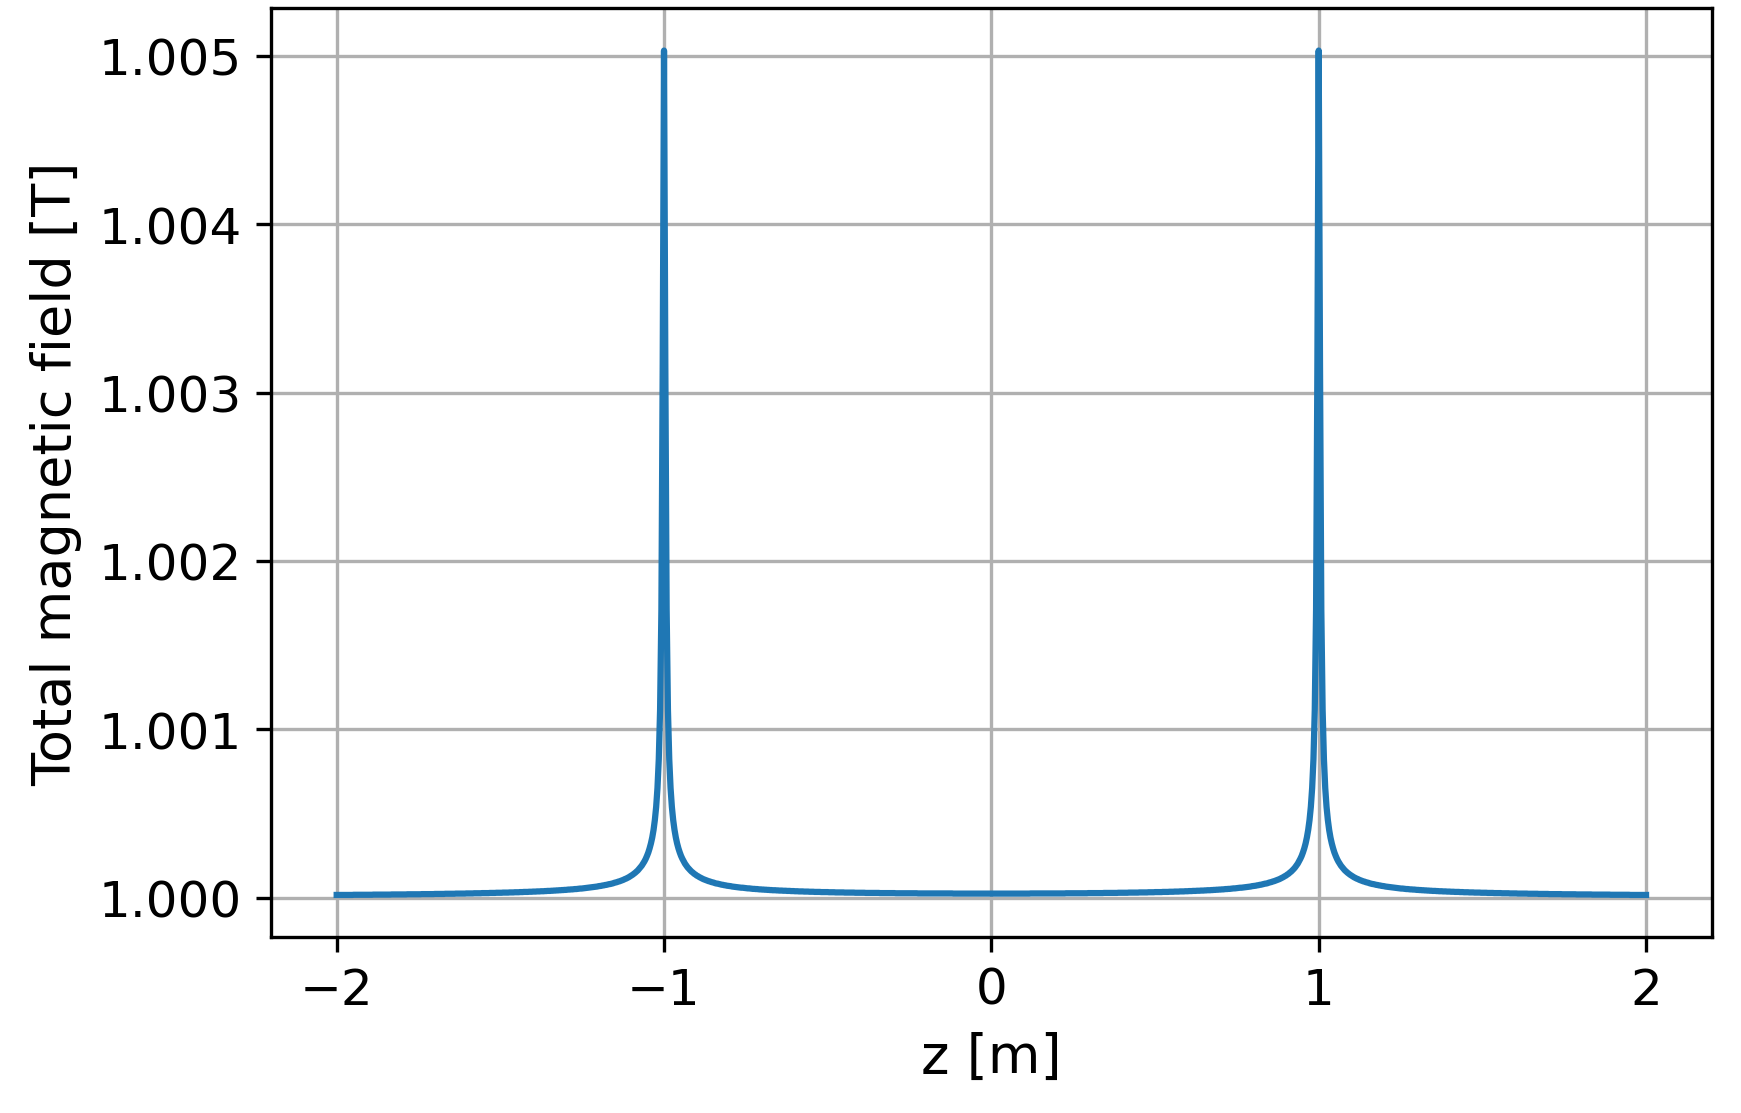
\includegraphics[width=77mm]{pictures/bathtubTrapCoils1_Width=0,1.png}
\vspace{-2mm}
\caption{Magnetic bathtub trap for a single coil at either end. Trap depth of this bathtub trap is $\Delta B=0.005$ T.}
\label{fig:bathtub1coil}
\end{figure}

Increasing the number of coils in the solenoids provides us with a perspective on how the solenoid coils should be distributed in a magnetic trap. \cref{fig:101coilsWidth=0.1} shows a magnetic trap where the width of the solenoids was constrained to $0.1\textrm{m}$. Using the calculation for the minimum pitch angle, the trap in \cref{fig:101coilsWidth=0.1} would constraint electrons with a pitch angle $\theta \geq 72.452^{\circ}$. It is shown from \cref{fig:101coilsWidth=0.2} that increasing width of the solenoid coils will have an undesired effect on our magnetic trap, because the trap depth has decreased, which will increase the constraint on our pitch angle to $\theta \geq 76.236^{\circ}$. Additionally, increasing the width of the solenoid coils will distort the uniform section of the trap further, which will have undesired effects on the electron's cyclotron motion.

\begin{figure}
    \centering
    \begin{subfigure}[b]{0.45\textwidth}
        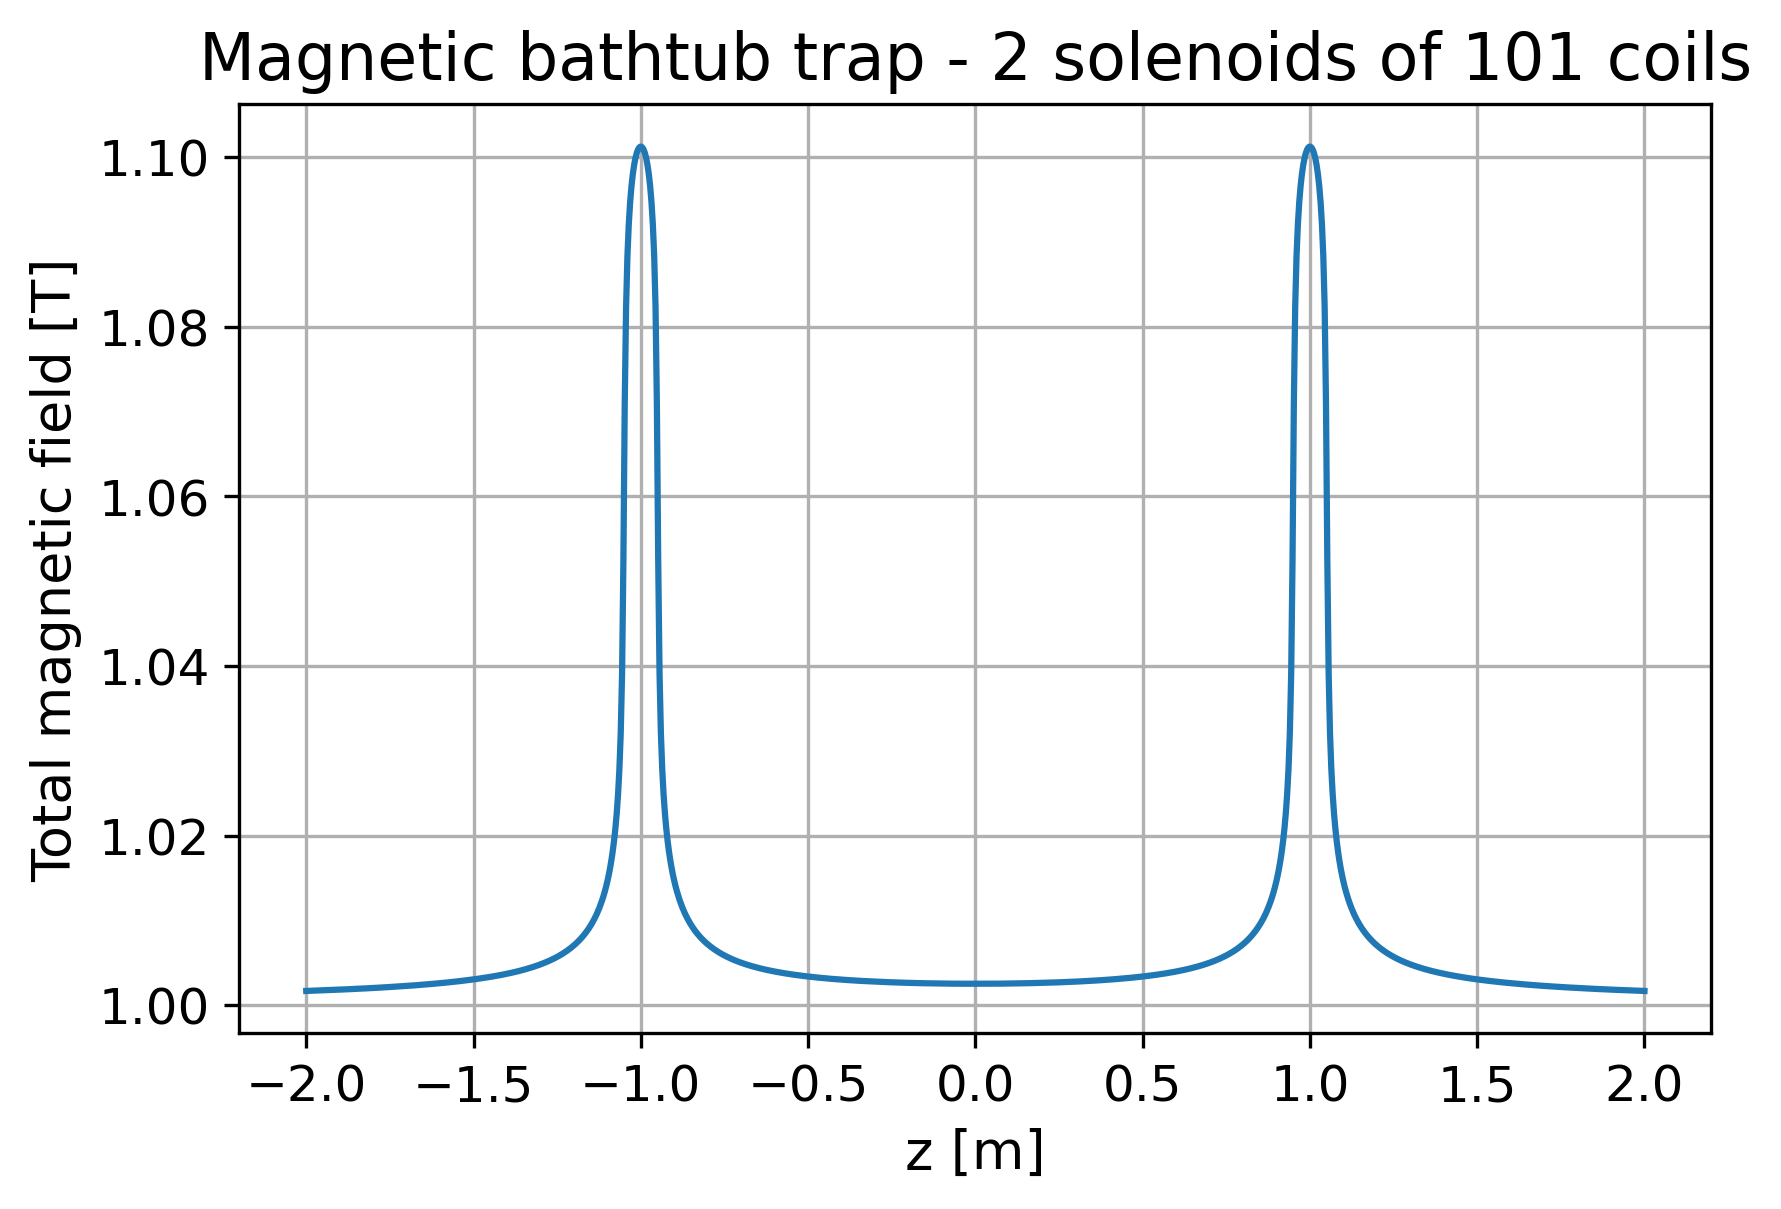
\includegraphics[width=77mm]{pictures/bathtubTrapCoils=101_Width=0,1.png}
        \caption{Magnetic trap with solenoids of width 0.1m. Trap depth $\Delta B=0.1$ T.}
        \label{fig:101coilsWidth=0.1}
    \end{subfigure} 
    \quad
    \begin{subfigure}[b]{0.45\textwidth}
        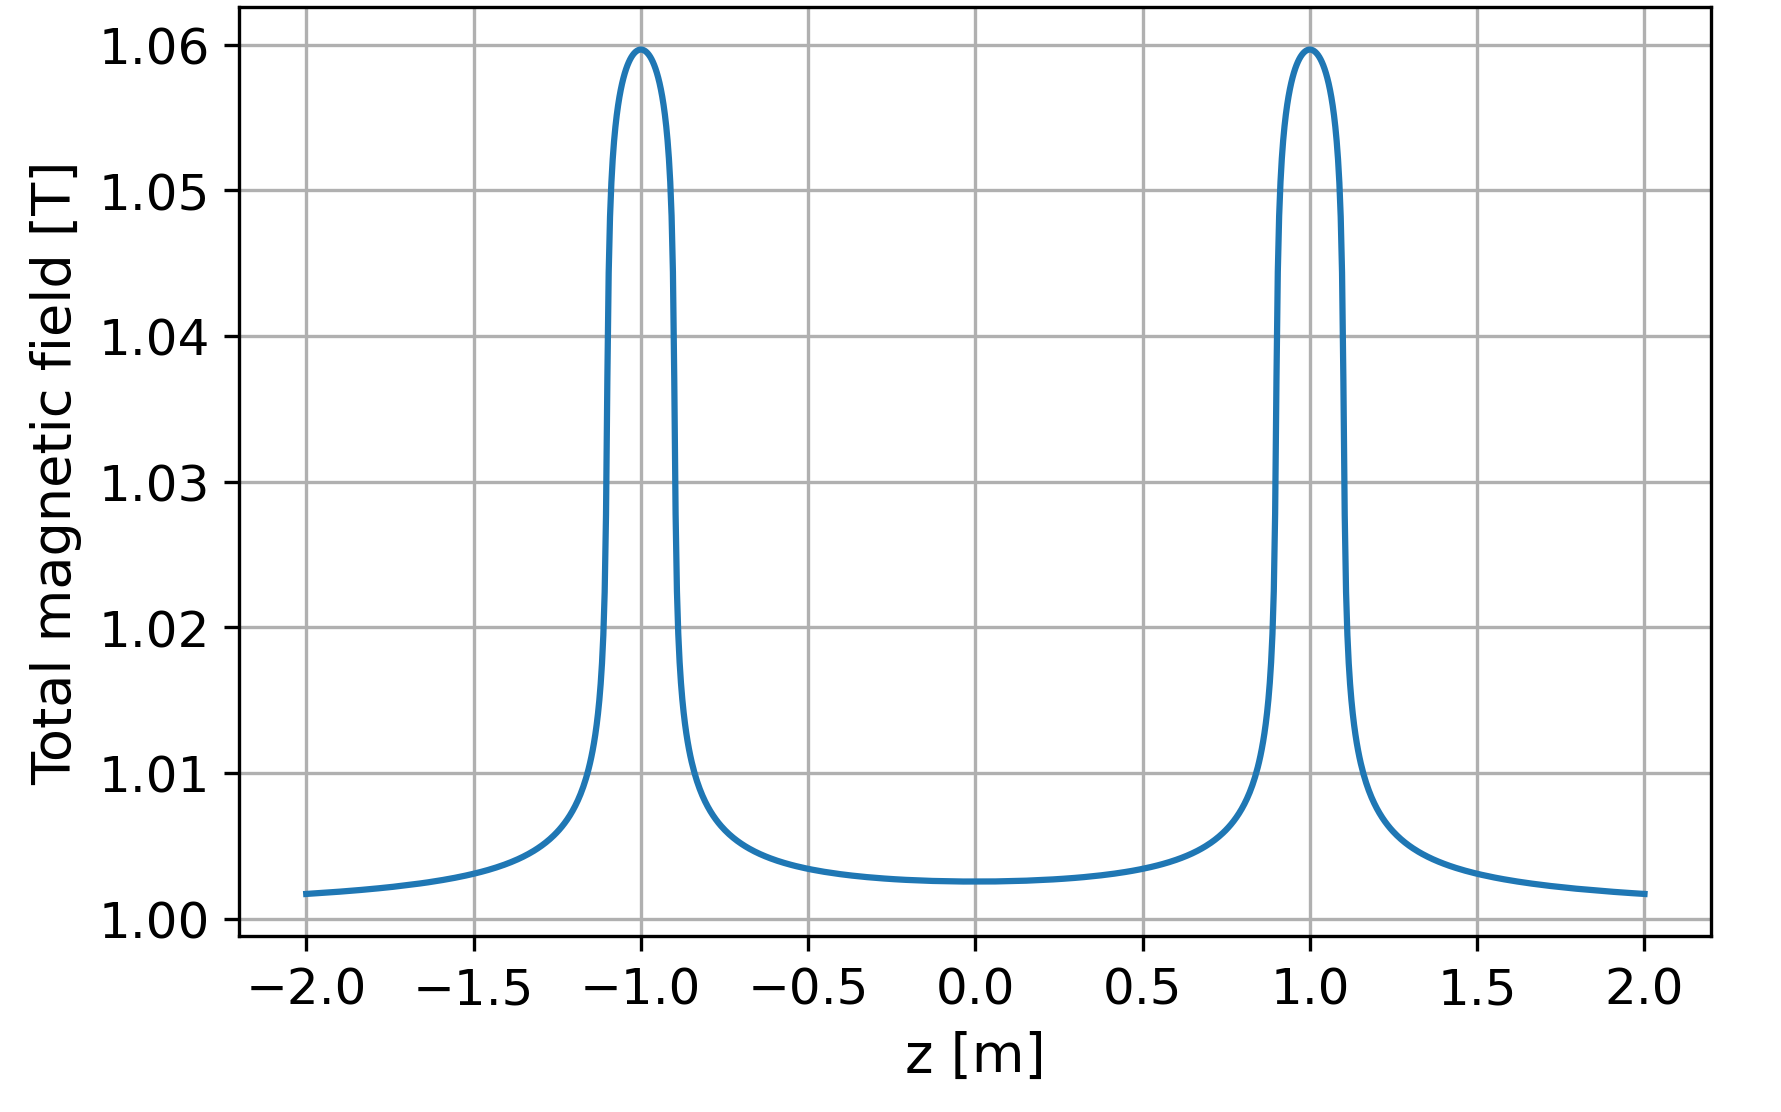
\includegraphics[width=77mm]{pictures/bathtubTrapCoils=101_Width=0,2.png}
        \caption{Magnetic trap with solenoids of width 0.2m. Trap depth $\Delta B=0.06$ T.}
        \label{fig:101coilsWidth=0.2}
    \end{subfigure}
\caption{Magnetic bathtub traps for 101 coils, with a width of 0.1m on the left, and a width of 0.2m on the right}
\label{fig:bathtub101coils}
\end{figure}

From studying the results obtained from the magnetic trap code, it is concluded that an optimal magnetic trap should contain multiple number of coils in the smallest width possible, in order to minimise distortion of the uniform field inside the trap, and maximise the potential barrier imposed by the solenoids on the electrons moving inside the uniform magnetic field. 
%------------------------------------------------------------------------
%------------------------------------------------------------------------
%------------------------------------------------------------------------
%------------------------------------------------------------------------
%------------------------------------------------------------------------
\subsection{Electron Trajectory}
The current working code considers only the Lorentz force when solving the trajectories of the electron. Running the code at a pitch angle of $87^{\circ}$, yielded an electron trajectory for a bathtub trap with a trap depth of $\Delta B = 0.003$ T, with 2 solenoid coils at $0.5$ and $-0.5$ m along the z axis. This pitch angle is just above the trap condition dictated by \cref{eq:pitchAngleCondition}. A snapshot of the trajectory at the start of the simulation is shown in \cref{fig:cyclo1}. For an energy of $18.575$ keV, the radius of gyration given by the Larmor radius, $r = \frac{m_{e}v}{eB}$ is $4.638\times10^{-4}$ m. This radius is maintained along the trajectory, demonstrating that the Boris algorithm conserves the energy of the system as required. Taking snapshots of the trajectory at the solenoid positions, \cref{fig:cyclo2} shows that the electron orbits become more tightly packed as the electron approaches the solenoid positions, indicating that the electron is bounced back into the magnetic trap due to the distortions imposed by the magnetic field.

If the pitch angle of the electron is decreased below the limit indicated by \cref{eq:pitchAngleCondition}, such as $84^{\circ}$, then the z component of the electron's velocity overcomes the magnetic trap with little change in the orbit spacing, and continues its cyclotron trajectory in the same z-direction, as shown in \cref{fig:cyclo4}. These results verify that the pitch angle condition is conserved in the simulations for the magnetic traps. Furthermore, the results confirm that a simulation utilising the Boris algorithm on the Lorentz equation of motion, in conjunction with the magnetic trap code, yields realistic results for an electron trajectory inside a magnetic trap.

\begin{figure}[t!]
\centering
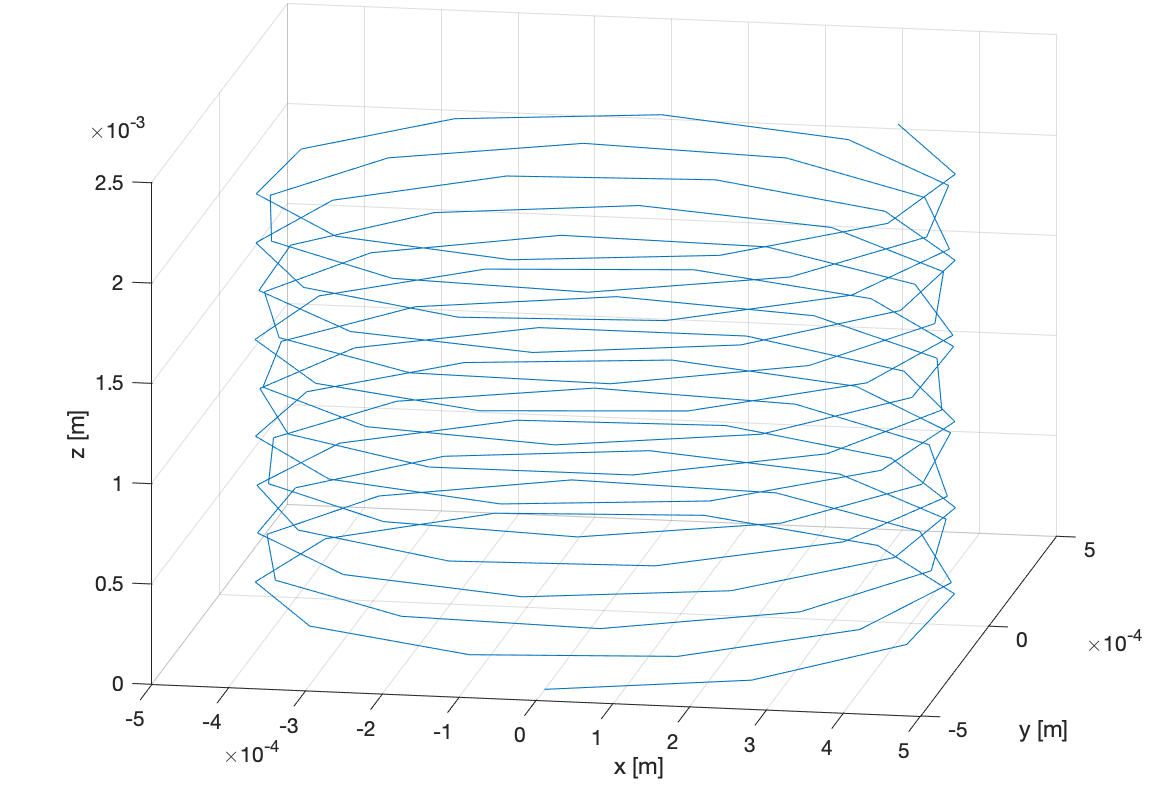
\includegraphics[width=77mm]{pictures/cyclotronMotion1.png}
\vspace{-2mm}
\caption{Cyclotron motion trajectory as calculated by the Boris algorithm.}
\label{fig:cyclo1}
\end{figure}

\begin{figure}[t!]
    \centering
    \begin{subfigure}[b]{0.45\textwidth}
        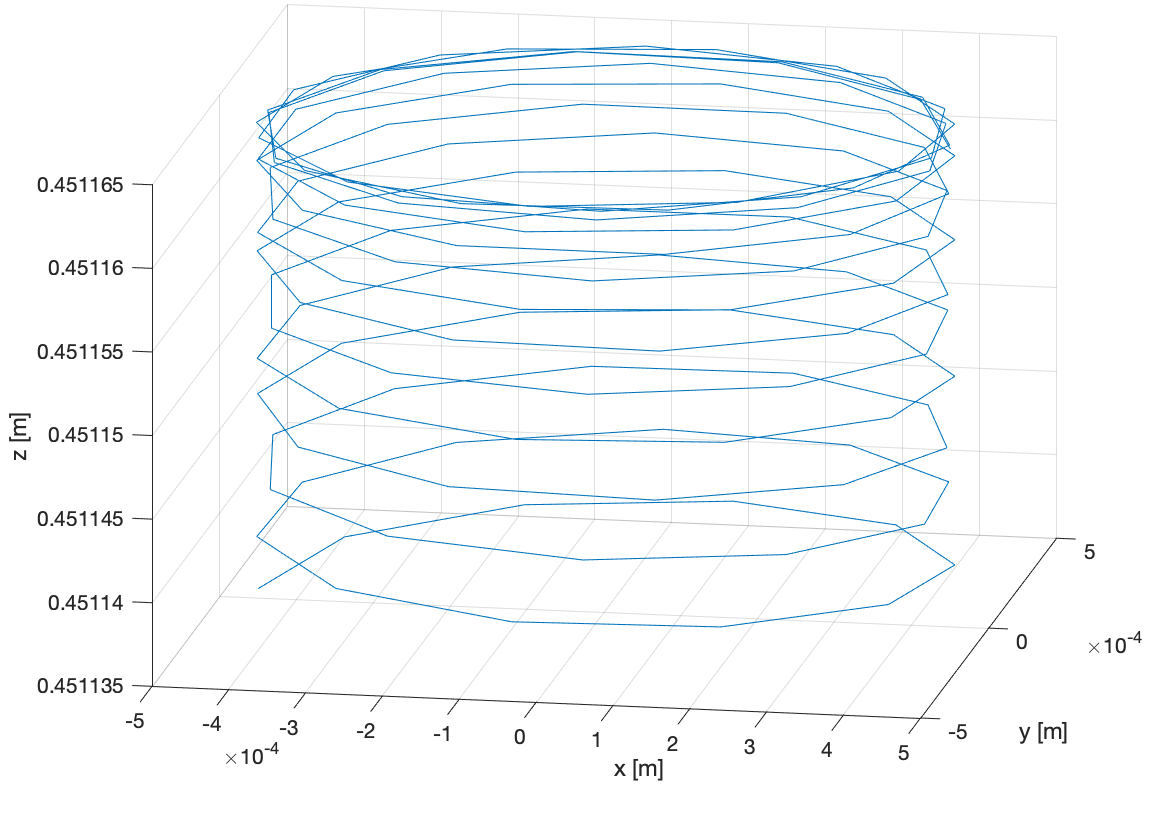
\includegraphics[width=77mm]{pictures/cyclotronMotion2.png}
        \caption{Solenoid position at $0.5$ m.}
        \label{fig:cycloBounce1}
    \end{subfigure} 
    \quad
    \begin{subfigure}[b]{0.45\textwidth}
        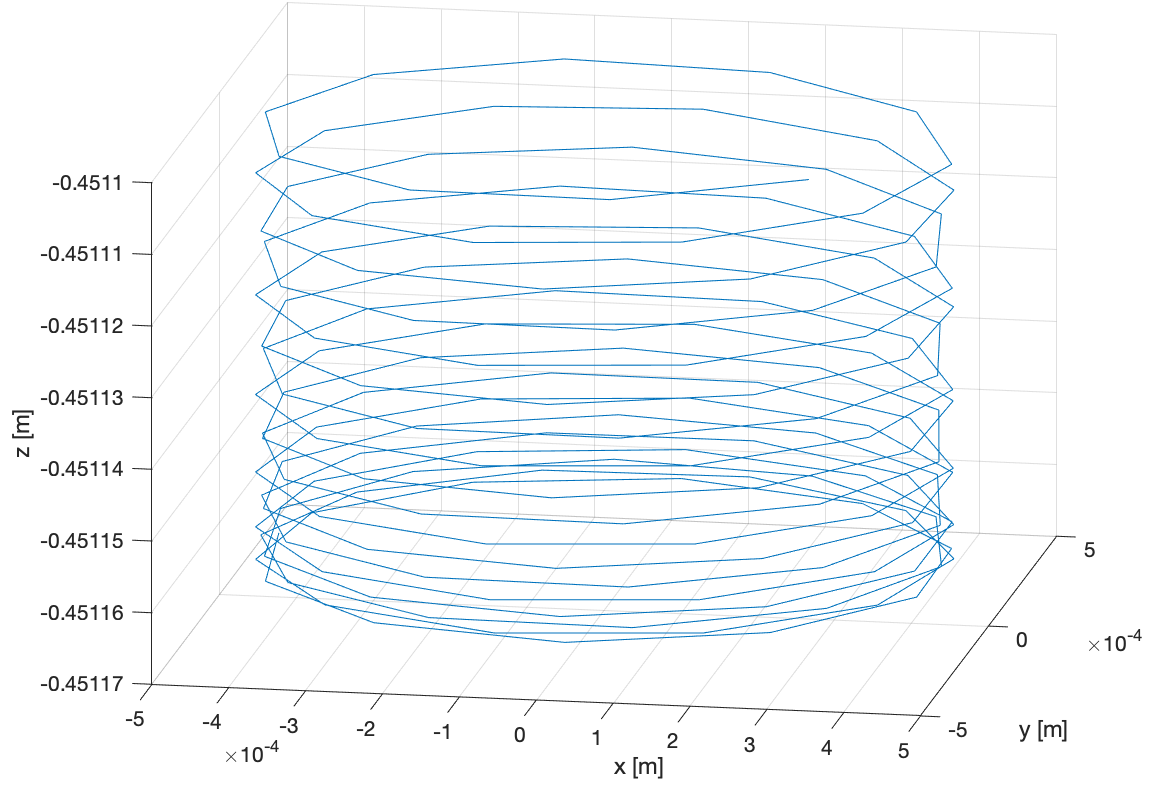
\includegraphics[width=77mm]{pictures/cyclotronMotion3.png}
        \caption{Solenoid position at $-0.5$ m.}
        \label{fig:cycloBounce2}
    \end{subfigure}
\caption{Electron trajectory bounced back into the magnetic trap near the two solenoid positions.}
\label{fig:cyclo2}
\end{figure}

\begin{figure}[t!]
\centering
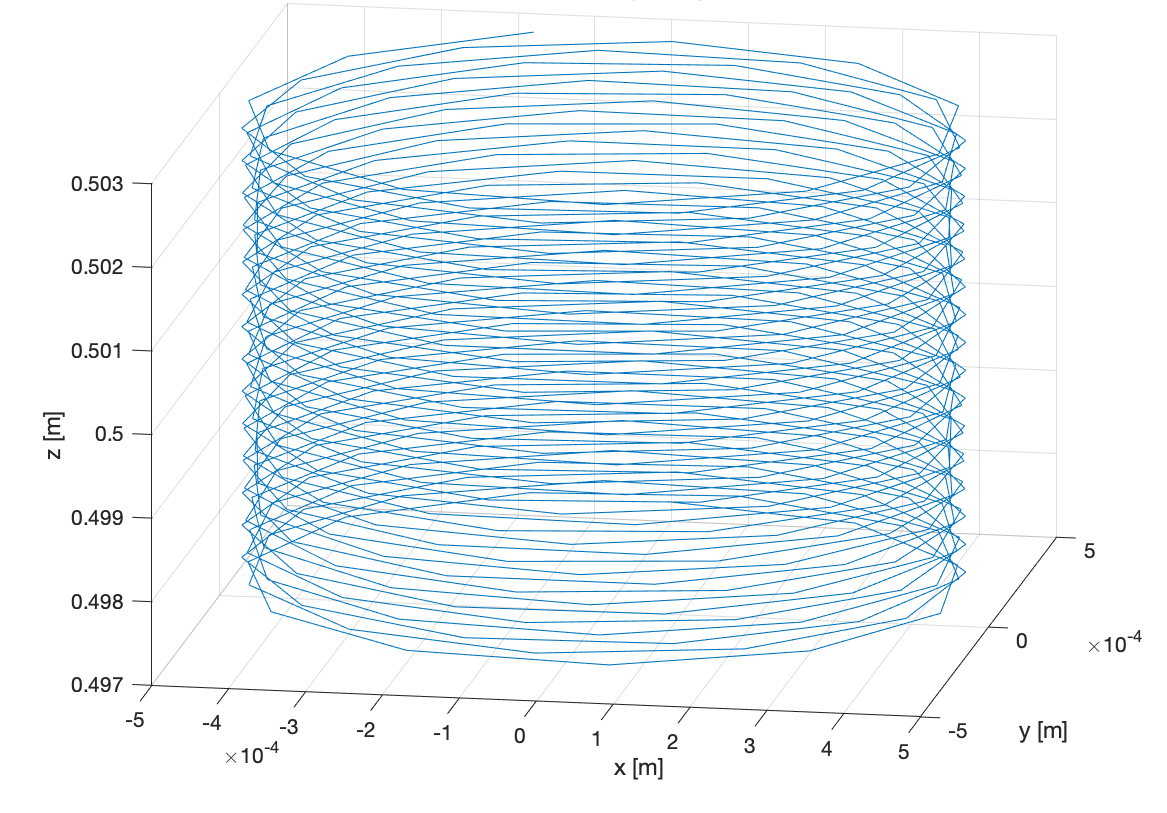
\includegraphics[width=77mm]{pictures/cyclotronMotion4.png}
\vspace{-2mm}
\caption{Cyclotron motion for a lower pitch angle. The electron overcomes the potential barrier imposed by the solenoid at a position of $z = 0.5$ m.}
\label{fig:cyclo4}
\end{figure}
%------------------------------------------------------------------------
%------------------------------------------------------------------------
%------------------------------------------------------------------------
%------------------------------------------------------------------------
%------------------------------------------------------------------------
\subsection{Electron Power Radiated}
The code using the Faraday tensor was unsuccessful in producing appropriate results. Considering that the equation is correct, it is hypothesised that a syntax error in the code is present which led to the wrong magnitude and shape of the curve, as the plot did not present the characteristic dimples of the lighthouse effect. Another suggestion as to why the Faraday tensor code produced the wrong result may be explained by the fact that computing the Poynting vector in the relativistic domain is not as simple as the cross product of the electric and magnetic field \cite{Paul2009,Lode2021}. The code implementing the Lienard-Wiechert equation was, however, successful in producing desired results. This code was implemented with an ideal cyclotron motion to verify that the power radiated over time produced the appropriate lighthouse effect from relativistic dynamics \cite{Jackson1999}. The code was successful in replicating the expected shape of the plot, as shown in \cref{fig:powerPlots1}, where in \cref{fig:powerPlot1} the phase of the motion stated is the angle between the electron position vector and the x axis (see \cref{fig:antenaSetup}). The antenna position defined in the simulation was $(0,0.05,0)$ m, which was 2 orders of magnitude above the radius of gyration ($4.638\times10^{-4}$ m), demonstrating that the circular motion of the electron had a very small effect on the magnitude of the power measured at the antenna. As the experimental setup proposed considers a stationary antenna as the primary apparatus with which to detect the power emitted, this method can only capture a small fraction of the total emitted power at any one time, which can explain why the power detected is 2 orders of magnitude below the expected result from previous experiments \cite{Ashtari2019}.

\begin{figure}
    \centering
    \begin{subfigure}[b]{0.45\textwidth}
        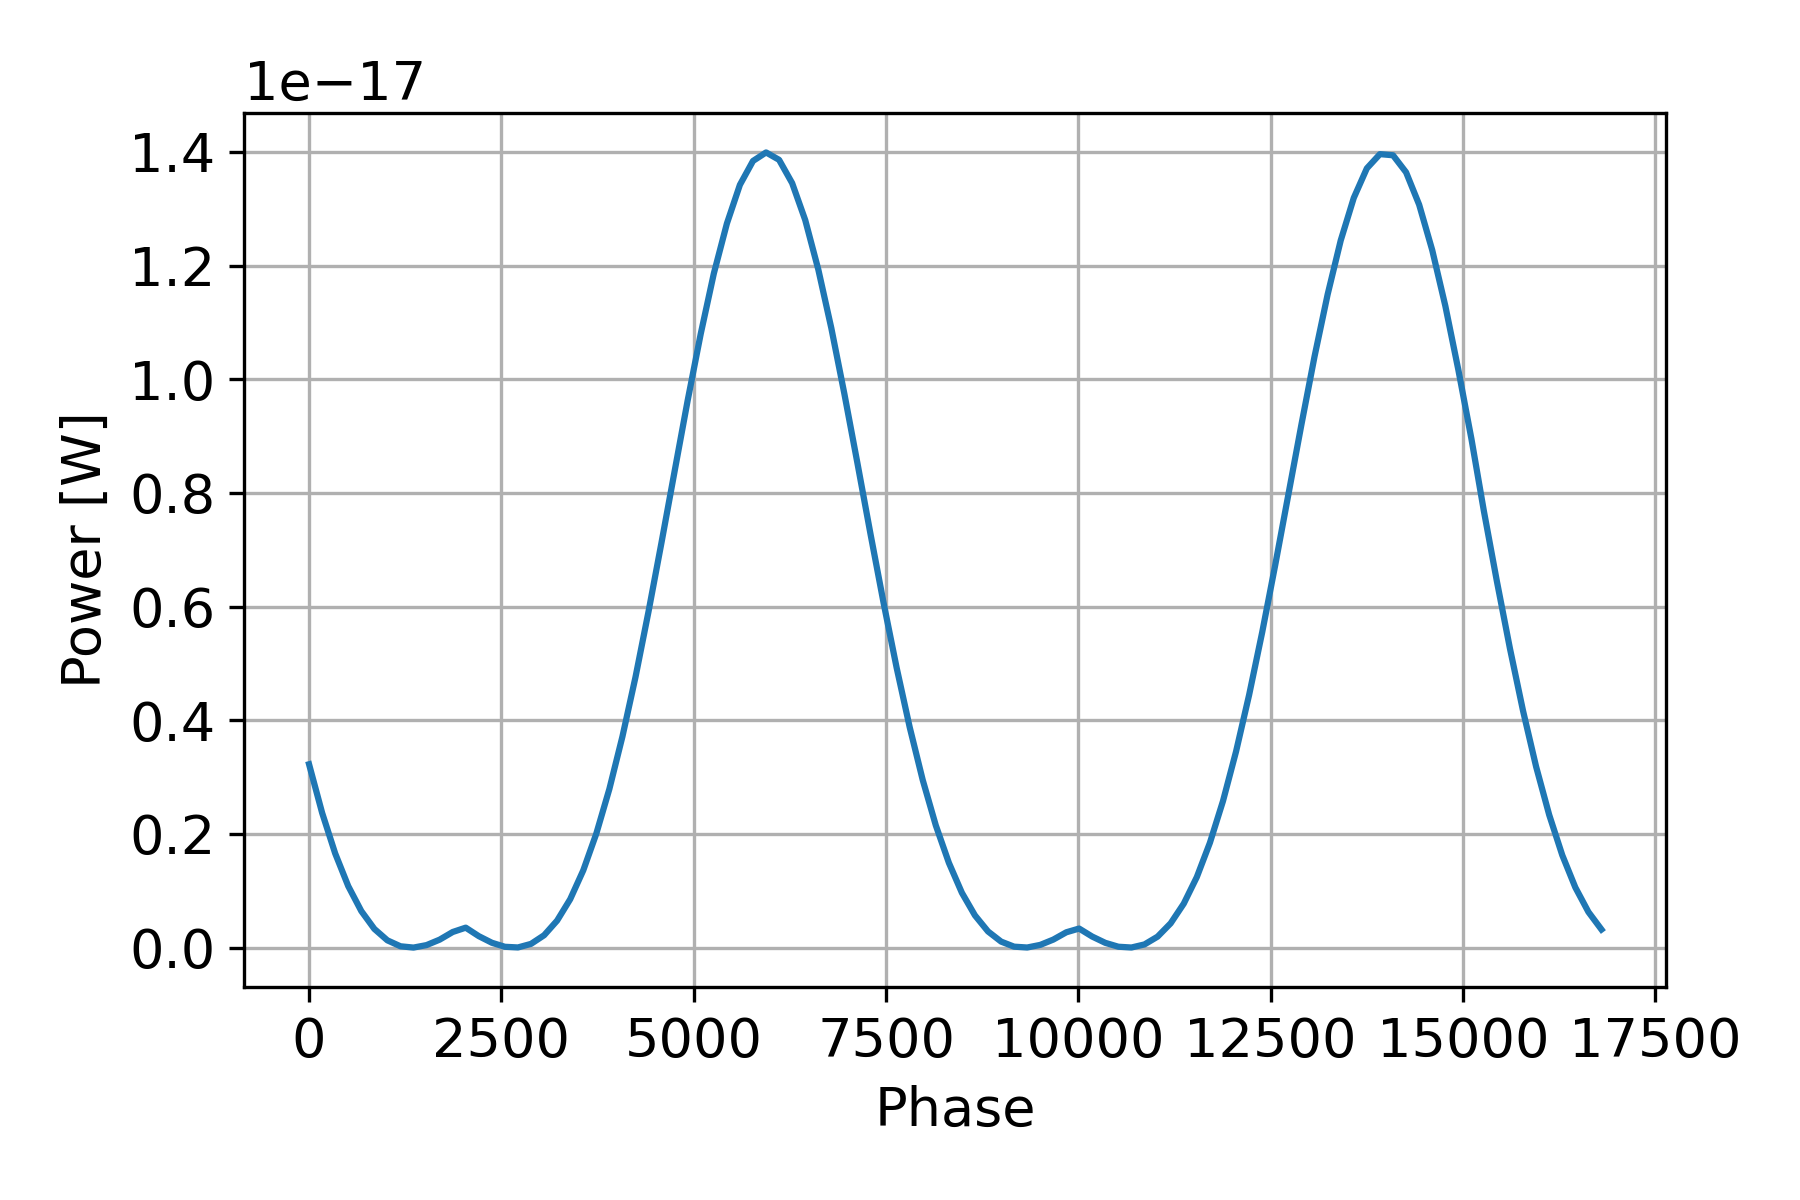
\includegraphics[width=77mm]{pictures/powerVsPhase.png}
        \caption{Power detected in fW vs phase of the motion.}
        \label{fig:powerPlot1}
    \end{subfigure} 
    \quad
    \begin{subfigure}[b]{0.45\textwidth}
        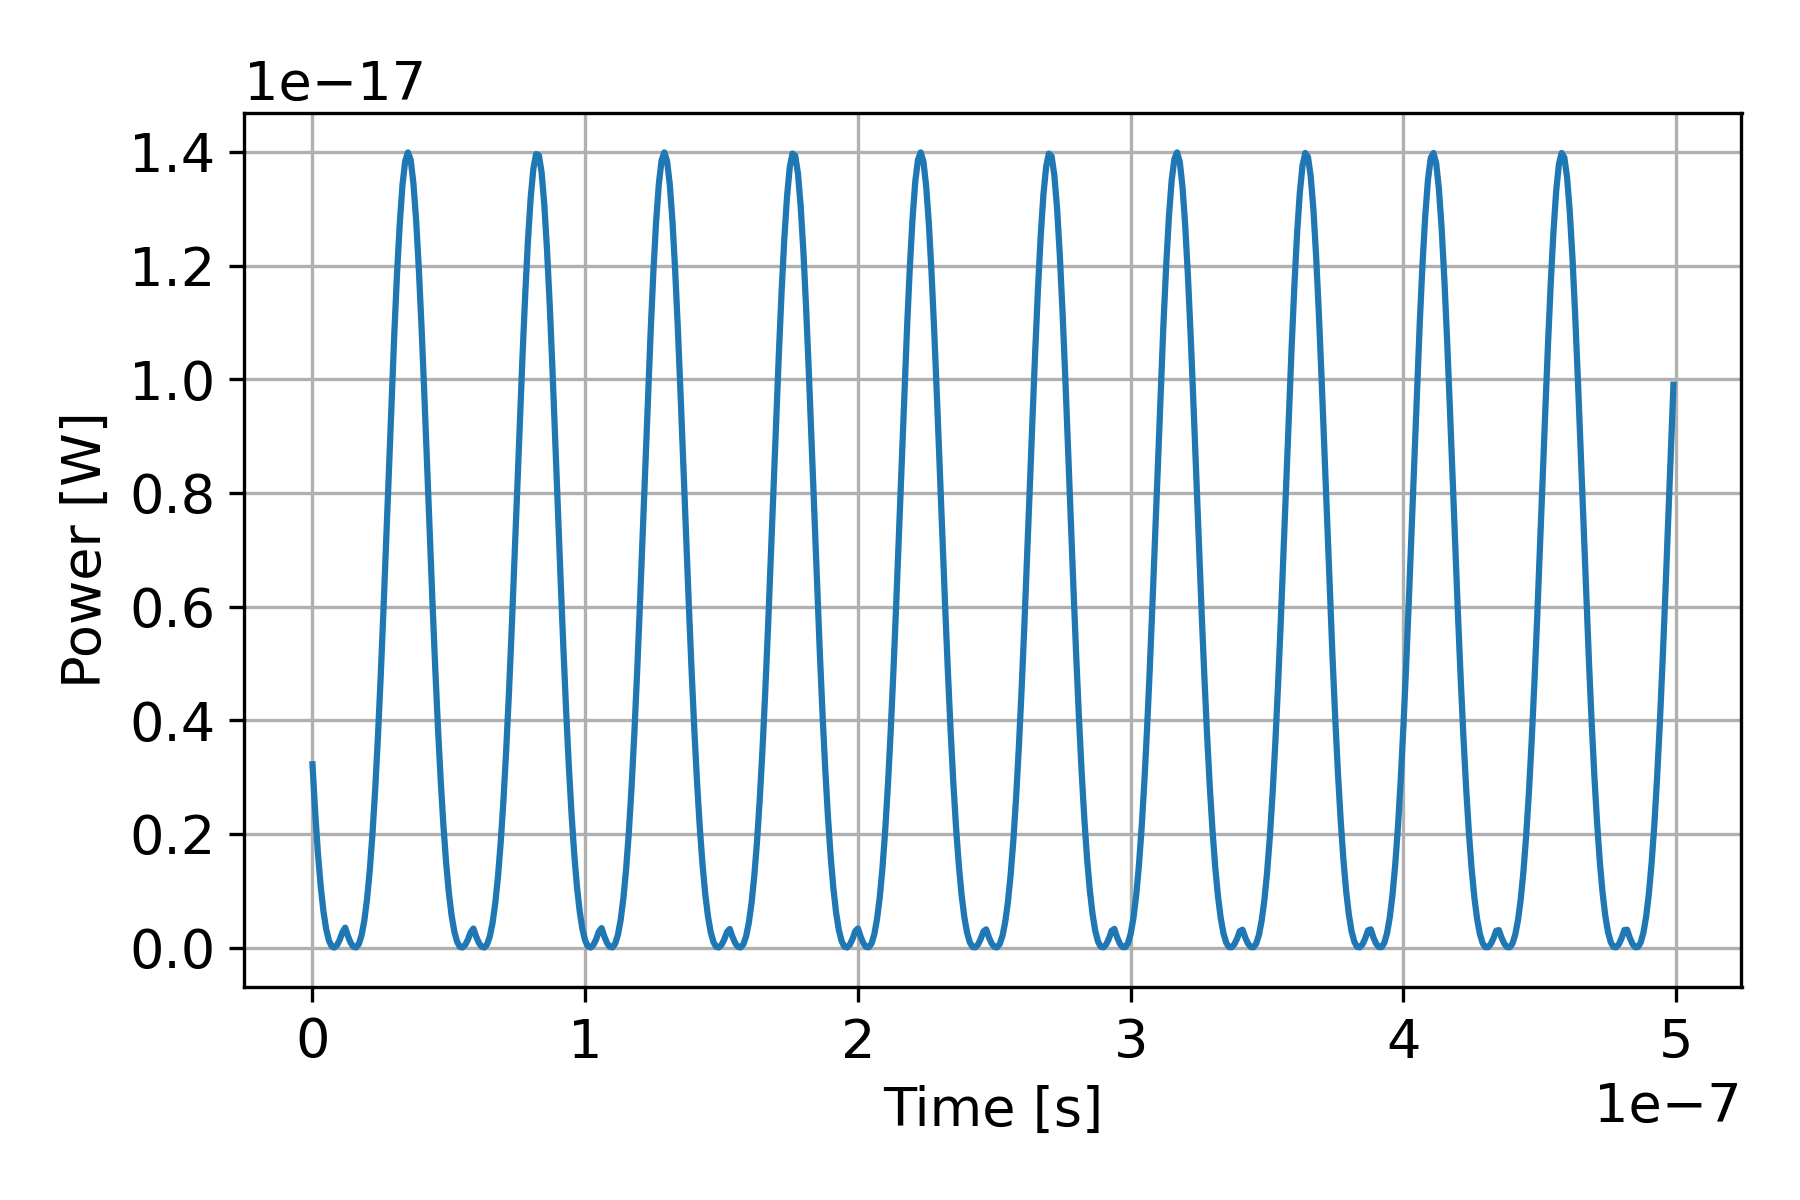
\includegraphics[width=77mm]{pictures/powerVsTime.png}
        \caption{Power detected in fW vs time in seconds.}
        \label{fig:powerPlot2}
    \end{subfigure}
\caption{Lienard-Wiechert formulation for the the power measured by an antenna.}
\label{fig:powerPlots1}
\end{figure}

With the cyclotron signal produced, a Fourier transform was applied to the data in order to ascertain the frequency of the signal. The Fourier transform returned a frequency of 5 GHz (see \cref{fig:fourierTransform}), which was not the desired frequency of 27.01 GHz for an electron with a kinetic energy of 18.575 keV. One explanation for this result is due to the simulation time-step implemented, at a time of $\Delta t = 1.0\times10^{-10}$, which would correspond to a sampling frequency of 10 GHz. Since the sampling frequency of a Fourier transform needs to be at least three to four times the frequency that needs to be extracted, this may explain the peak of the frequency at 5 GHz. To this end, future simulations should utilise a time-step below $\Delta t = 9.09\times10^{-12}$ in order to detect a signal at the desired value of 27.01 GHz. The sampling frequency needs to be more than twice the signal frequency because the signal returned should return a central peak along with sidebands of frequency due to phase shift phenomena in the power emitted \cite{Ashtari2019}.

\begin{figure}[b!]
\centering
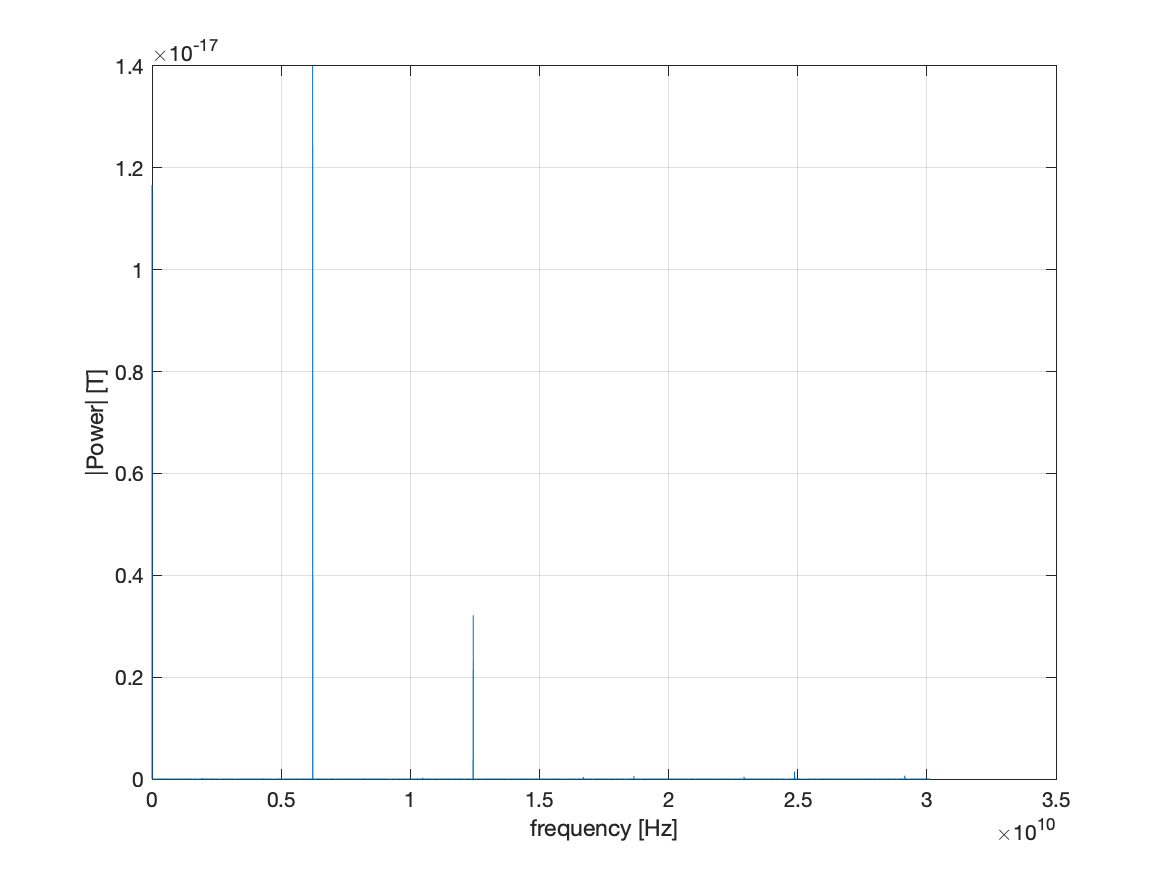
\includegraphics[width=77mm]{pictures/transform.png}
\vspace{-2mm}
\caption{Fourier transform of the signal detected, with a peak frequency of 5 GHz at a power of $1.4\times10^{-17}$.}
\label{fig:fourierTransform}
\end{figure}
%------------------------------------------------------------------------
%------------------------------------------------------------------------
%------------------------------------------------------------------------
%------------------------------------------------------------------------
%------------------------------------------------------------------------
\subsection{Lock-in Amplifier}
%On the lock-in amplifier, in case you can't get results since the tool isn't working yet then you can state that and discuss the status, i.e. which part isn't working and what is working preferably with demonstrations in figures. After all, the report is a reflection of your work up to the time of writing. 
The lock-in amplifier code was unable to return a complete simulation for detecting an unknown signal within noise. One reason as to why this may the case is because the number of lock-in amplifiers used to scan the signal were not enough (around 100) to completely scan the entire frequency domain of importance. The method is unable to detect the exact signal because it is scanning a discrete number of points over a much larger discrete set of points imposed by the randomise function on the signal frequency, so the code is entirely dependent on how small the time-step is in the simulations. The method could mathematically be improved by increasing the number of lock-in amplifiers that are used to scan the bandwidth of interest, but this would not be a practical implementation into real life situations. Additionally, in real life situations, the domain that is scanned would have the additional issue of being a continuous domain, which will affect the detection of an unknown signal even more harshly. 
%One solution to this problem could be to model the frequency shift as a function of time, which would become the reference frequency of the lock-in amplifier as the frequency shifts
%------------------------------------------------------------------------
%------------------------------------------------------------------------
%------------------------------------------------------------------------
%------------------------------------------------------------------------
%------------------------------------------------------------------------
\section{Conclusion}
In this report it has been shown that the electron motion inside a magnetic bathtub trap can be accurately simulated in order to measure its power radiated as a function of the electron's position. Some results on the magnetic trap have clarified that an optimal trap should have solenoid coils tightly packed in order to minimise the distortion of the uniform field inside the trap, and maximise the potential barrier that electrons will need to overcome in order to escape the magnetic trap. The results on trajectories calculated have validate the limit on the pitch angle that the cyclotron motion should have in order for electrons to be contained inside.
The figures on the power received at an antenna have validated that simulations produce the proper lighthouse effect of relativistic electromagnetic radiation. As this report is based on a recently established and ongoing project, the final report and its goals have been constantly redefined due to developments in the project. %The theoretical concept of measuring an electron's cyclotron frequency to extract its energy has 
%------------------------------------------------------------------------
%------------------------------------------------------------------------
%------------------------------------------------------------------------
%------------------------------------------------------------------------
%------------------------------------------------------------------------
\section{Further Discussion}
%You should be drawing conclusions as you discuss your results but this section acts as a summary. Many people will read the conclusion first to get a feel for the quality of the results, etc. So this can be an important section.
The results obtained have successfully replicated an electron trajectory in a magnetic trap when the Lorentz force is considered. Further work that could be implemented may consider the motion of the electron when the Abraham-Lorentz force is included, for which code was produced but was erroneous in results. Additionally, it is suggested that future work may include trajectories where the energy loss due to the power emitted is accounted for. This consideration will be particularly important in detecting the frequency of the electron, since a shift energy will result in a shift of frequency. For such a consideration, the usual method of applying a lock-in amplifiers will not be appropriate because the frequency of the signal will constantly change. A suggestion as to how this problem may be tackled implements a changing reference signal that may be controlled using an appropriate analytical equation for the rate of energy loss of the electron as a function of time, so that the reference frequency shifts side by side with the signal frequency. \\
More results on the power radiated for different trajectories would elucidate the behaviour of the power detected at an antenna, as the electron oscillates inside the magnetic trap. This will be particularly useful to understand because the magnitudes of the power received are already very small, and will only become smaller as an electron oscillates perpendicularly past an antenna. \\
Future work that could be implemented may revise the code on the power measured, in order to ascertain if the signal received is erroneous since its Fourier transform yielded an unexpected result. Moreover, trajectories with a smaller time-step could be simulated in order to verify if the error lies in the code or in the sampling rate of the Fourier transform.
Further additions into the simulation framework could include the change in frequency of an electron due to a changing magnetic field, since a bathtub trap does not have an exactly homogeneous field, particularly at the extremities. To this end, \cref{cyclotronFrequency} might be modified in order to include a magnetic field as a function of time, so that the value of the frequency can be more accurately calculated for a given position at a point in time \cite{Ashtari2019}. \\
%This is also my place to remind you of the length limits. For MPhys/MMathPhys, you are recommended to aim for a length of 25 pages; the absolute limit is 30 pages with ONLY your bibliography (aka references list) being allowed to spill beyond that.


\printbibliography

\end{document}
